\documentclass[12pt]{article}
\usepackage[utf8]{inputenc}
\usepackage{xcolor}
%\usepackage{mdframed}% for framed figures
%\colorlet{framecolor}{gray}

\usepackage{natbib} 
\usepackage{ulem}%for strike through, can be deleted when submitting the paper
%\usepackage[backend=bibtex, style=authoryear]{biblatex} %compile on this order --> LaTeX BiBTeX LaTeX
%\addbibresource{refs.bib}
\usepackage{amsmath,amsthm,amsfonts,dsfont}
\usepackage{mathrsfs}  
\usepackage{tikz}
\usepackage{amssymb}
\usepackage{fullpage}
\usepackage{tabularx}
\usepackage[hidelinks]{hyperref}
\usepackage{float}
\usepackage{subfigure}
\newtheorem{theorem}{Theorem}[section]
\newtheorem{example}{Example}[section]
\newtheorem{property}[theorem]{Property}
\newtheorem{properties}[theorem]{Properties}
\newtheorem{corollary}[theorem]{Corollary}
\newtheorem{lemma}[theorem]{Lemma}
\theoremstyle{definition}
\newtheorem{definition}{Definition}[section]
\theoremstyle{remark}
\newtheorem{remark}{Remark}


\usepackage[inline]{enumitem}

\newcommand{\restrict}{\mid}
\newcommand{\range}[1]{\mathscr{#1}}

%%%%%%%%%%%%%%%%%%%%%%%%%%%%%%%%%% Greek
\newcommand{\zdistparama}{\alpha}
\newcommand{\zdistparamb}{\beta}
\newcommand{\zdistparamc}{\gamma}
\newcommand{\freeGamma}{\Gamma}
\newcommand{\order}{\delta}
\newcommand{\freeDelta}{\Delta}

\newcommand{\dominantU}{\nu}
\newcommand{\dominantUbar}{\bar{\nu}}
\newcommand{\sampledensity}{\mathbf{\pi}}
\newcommand{\intensity}{\lambda}
\newcommand{\Intensity}{\Lambda}
\newcommand{\dominantY}{\eta}
\newcommand{\dominantYbar}{\bar{\eta}}
\newcommand{\intensityratio}{\rho}
\newcommand{\densityratio}{\rho}
\newcommand{\parampop}{\theta}
\newcommand{\permutation}{\tau}
\newcommand{\paramnuisance}{\xi}
\newcommand{\provar}{\Sigma}
\newcommand{\Residual}{\varepsilon}
%\newcommand{\Covf}{\Gamma}
%%%%%%%%%%%%%%%%%%%%%%%%%%%%%%%%%% Latin

\newcommand{\acos}{acos}
\newcommand{\subsetA}{A}
\newcommand{\Covariogram}{C}
\newcommand{\cardinality}{\mathrm{cardinality}}
\newcommand{\Cov}{\mathrm{Cov}}
\newcommand{\derive}{\mathrm{d}}
\newcommand{\Design}{D}
\newcommand{\design}{\mathbf{d}}
\newcommand{\E}{\mathrm{E}}
\newcommand{\density}{\mathrm{f}}
\newcommand{\Semivariogram}{G}
\newcommand{\indicator}{I}
\newcommand{\nrep}{J}
\newcommand{\repindex}{j}
\newcommand{\Sampleindex}{K}
\newcommand{\sampleindex}{\mathbf{k}}
\newcommand{\likelihood}{\mathscr{L}}
%\newcommand{\popsize}{N}
\newcommand{\uple}{m}
\newcommand{\Samplesize}{N}
\newcommand{\samplesize}{\mathbf{n}}
%\newcommand{\P}{P}
\newcommand{\Sample}{S}
\newcommand{\sample}{\mathbf{s}}
\newcommand{\size}{\mathrm{size}}
\newcommand{\Pop}{\mathrm{U}}
\newcommand{\toPop}{\bar{\mathrm{U}}}
\newcommand{\Var}{\mathrm{Var}}
\newcommand{\Position}{X}
\newcommand{\position}{\mathbf{x}}
\newcommand{\SignalSpace}{\mathscr{Y}}
\newcommand{\toSignalSpace}{\bar{\SignalSpace}}
\newcommand{\Signal}{Y}
\newcommand{\signal}{\mathbf{y}}
\newcommand{\Desvar}{Z}
\newcommand{\DesvarSpace}{\mathscr{Z}}
\newcommand{\desvar}{\mathbf{z}}

\newcommand{\xxx}{.5}
\newcommand{\yyy}{.5}
\newcommand{\hhh}{.5}
\newcommand{\xx}[1]{\renewcommand{\xxx}{#1}}
\newcommand{\hh}[1]{\renewcommand{\hhh}{#1}}
\newcommand{\yy}[1]{\renewcommand{\yyy}{#1}}


\newlength{\defbaselineskip}
\setlength{\defbaselineskip}{\baselineskip}
\newcommand{\setlinespacing}[1]%
           {\setlength{\baselineskip}{#1 \defbaselineskip}}
\newcommand{\doublespacing}{\setlength{\baselineskip}%
                           {2 \defbaselineskip}}
 \newcommand{\singlespacing}{\setlength{\baselineskip}{1.3 \defbaselineskip}}




\newcommand\smallplot{
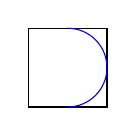
\begin{tikzpicture}
    \draw (0, 0) rectangle (1, 1);
    \draw[blue] (\xxx,\yyy+\hhh) arc(90:-90:\hhh);
  \end{tikzpicture}}

\title{The effect of Informative Selection on the estimation of parameters related to Spatial Processes}
\date{}
\author{Daniel Bonn\'ery \thanks{Epidemiology and Modelling Group, Department of Plant Sciences, University of Cambridge, UK} \and Francesco Pantalone\thanks{Department of Economics, University of Perugia, Italy} \and M. Giovanna Ranalli\thanks{Department of Political Science, University of Perugia, Italy}}


\begin{document}
\normalem %delete this line when ulem packages is removed

\maketitle

%\tableofcontents

\begin{abstract}
This paper extends the concepts of informative selection, population distribution and sample distribution to a spatial process context. These notions were first defined %by \cite{pfefferman_1992}
in a context where the output of the random process of interest consists of independent and identically distributed realisations for each individual of a population. %{\color{red} \cite{bonnery2012uniform}}
It has been showed that informative selection induces stochastic dependence among realisations on selected units. In the context of spatial processes, the ``population'' is a continuous space and realisations for two different elements of the population are not independent. %We show how informative selection may induce a different dependence among selected units, how the sample distribution differs from the "population" distribution, and how one can  account for this effect in an simulated study when doing statistical inference, including Semi-variogram parametric and semi parametric estimation, as well as prediction on the part of the space for which the random process was not observed.
We show how informative selection may induce a different dependence among selected units from a spatial process and how the sample distribution differs from the population distribution. %and how one can account for this effect in order to avoid biased estimates. %in an simulated study when doing statistical inference about the variogram.
%In particular, we provide a first solution on how to account for  informative selection in doing statistical inference about the variogram. %, and when a finite population is considered.

%We show how informative selection may induce a different dependence among selected units and how the sample distribution differs from the ``population'' distribution. We then focus on estimation of the variogram, and we provide a first solution to how account for the informative selection.
~\\
\textbf{Keywords}: analytic inference, point process, sample distribution, population distribution, sample likelihood, unequal probability sample, variogram.

\end{abstract}

\singlespacing

\section{Introduction} \label{sec:intro}
Spatial processes are employed in many fields, like geology, Earth science, environmental and agricultural surveys, among many others. A huge variety of data can be employed, such as rainfall data \citep{ord1979spatial}, atmospheric data \citep{thiebaux1987spatial}, forestry data \citep{samra1989spatial} and soils data \citep{burgess1980optimal} {\color{red} FP: these references are a little bit old, so not sure if we can leave it}. In these applications, a general approach is to postulate a spatial process for the variable $\Signal$ under investigation, that is a stochastic process which is assumed to have generated the population values, also called \emph{superpopulation} model. %Such process is usually parametric, i.e. characterized by a finite number of parameters $\boldsymbol{\theta}$, and the interest is on inference about such parameters. If we use sample data in order to make inference about $\boldsymbol{\theta}$,
When using sample data, we need to pay attention at the relation between the spatial process and the mechanism selection. Indeed, the distribution of the observed data can be different from the distribution assumed for the population by means of the spatial process. In other words, the density obtained by the sample data may not be the density obtained by reducing the number of terms in $P^{\Signal}$, as if the units were selected completely at random. In this case, we say that the sampling is \emph{informative}. Ignoring an informative sample may lead to biases and erroneous inference, as illustrated for example in \cite{skinner1989analysis}. This could happen when there is dependence between the assumed stochastic model and the sampling mechanism, that is the units are selected dependently to the variable of interest. Examples of this type of mechanism selection are, among many others, length-biased sampling, endogenous stratification, adaptive sampling, sequential quota sampling and cut-off sampling. For more details, see Section 3 of \cite{bonnery2012uniform}.
\\ When dealing with spatial processes, an important tool is the \emph{variogram}, which analyzes the degree of spatial dependence of such processes and provides useful insights on the phenomenon under investigation. For instance, the variogram is the key component for the well-known \emph{kriging} method \citep{matheron1962traite}, and it plays a crucial role on prediction since it is used to compute the kriging weights. 
\\ In this paper, we study the effect of informative selection when the variogram is of interest. We consider informative selection as a situation where the sample responses, given that they were selected, are not i.i.d. from the superpopulation model. As in \cite{pfeffermann1998parametric}, we start from the distribution of the observed values given they were selected, or \emph{sample pdf}. The major difference in our approach is that, while \cite{pfeffermann1998parametric} consider the observations as if they were independently distributed according to the sample pdf, our work consider the dependence between the observed units. We provide a theoretical background for the definitions of \emph{population variogram} and \emph{sample variogram}, and some properties of the \emph{naive} estimator, i.e. the estimator that does not take into account the informativeness of the selection mechanism.
\\The paper is organized as follow. In Section \ref{sec:stat_fra} we define the statistical framework used throughout the paper. In particular, general notions and the concepts of spatial process, sample, design and design variables are introduced. In Section \ref{sec:sampledistribution} the sample distribution and the population distribution are defined, and in Section \ref{sec:estimation} estimation of the variogram is analyzed and properties of the naive estimator are presented. Finally, Section \ref{sec:con} provides conclusion and future research.

% The \emph{sample pdf} is defined as the conditional distribution of the random variable $\Signal$ given that it was selected. \cite{pfeffermann1998parametric} use a sample likelihood approach to inference for the superpopulation model, where the product of the sample pdfs is maximized, as if the responses were iid.

%The major approaches to analytic inference from survey data are all based on the likelihood concept. The maximum \emph{full-information} likelihood approach defines the likelihood as the probability of observing all the relevant data available \citep{breckling1994maximum} and the process that has to be accounted for is given by the joint distribution of the spatial process $\Signal$ and the selection mechanism, while the maximum \emph{sample-likelihood} focuses on the distribution of $\Signal$ given it was observed \citep{krieger1992maximum, pfeffermann1993role, pfeffermann1998parametric, pfeffermann1999parametric}, and if this conditional distribution differs from the marginal distribution of $\Signal$, selection bias is introduced and the mechanism selection is \emph{informative}.
 %Since just a portion of the population is observed, the relevant likelihood is given by $P^{I_{U},\Signal_{S}}=\int{P^{I_{U},\Signal_{U}}d\Signal_{U \backslash s}}$, which is usually different from $P^{S}=\int{P^{\Signal_{U}}d\Signal_{U \backslash s}}$.

%The major approaches to analytic inference from survey data are all based on the likelihood concept. The maximum \emph{full-information} likelihood approach defines the likelihood as the probability of observing all the relevant data available \citep{breckling1994maximum}. The process that has to be accounted for is given by the joint distribution of the spatial process $\Signal$ and the selection mechanism.%Since just a portion of the population is observed, the relevant likelihood is given by $P^{I_{U},\Signal_{S}}=\int{P^{I_{U},\Signal_{U}}d\Signal_{U \backslash s}}$, which is usually different from $P^{S}=\int{P^{\Signal_{U}}d\Signal_{U \backslash s}}$.
% \\ The maximum \emph{sample-likelihood} focuses on the distribution of $\Signal$ given it was observed \citep{krieger1992maximum, pfeffermann1993role, pfeffermann1998parametric, pfeffermann1999parametric}. If this conditional distribution differs from the marginal distribution of $\Signal$, selection bias is introduced and the mechanism selection is \emph{informative}.


\section{Statistical Framework} \label{sec:stat_fra}
This section illustrates the concepts and notations defined in \cite{dbb1}.
\subsection{General notations}

In this paper, all random variables are defined on a probability space $(\Omega,\mathscr{A},P)$. The expected value and variance/covariance operators are defined with respect to the probability measure $P$. 
For two sets $E$ and $F$, $(E\to F)$ or $F^E$ designate the set of the functions from $E$ to $F$.
The notation "$g:E\to F,x\mapsto g(x)$" means: let $g$ be a mapping from set $E$ to set $F$ that to $x$ associates $g(x)$. For $f:E\to (F\to G)$, $g:E\to F$, $h:E\to (H\to F)$,  the notation $f[g]$ designates the function :  $f[g]:E\to G$, such that $f[g](x)=(f(x))(g(x))$, and the notation 
$f[h]$ designates the function :  $f[h]:E\to (H\to G)$, such that $f[h](x)=(f(x)\circ h(x))$.


For a set $E$, $\bar{E}$ designates the set $\{\mathbf{0}\}\cup\bigcup_{n\in\mathbb{N},n\geq 1} E^{\{1,\ldots,n\}}$, where $\mathbf{0}=E^\emptyset$ corresponds to the set containing an application with empty domain.
Let denote by $\size $ the application that maps an application to the cardinality of its domain: $\bar{E}\to\mathbb{N}$, $\mathbf{e}\mapsto n$ if $\position\in E^{\{1,\ldots,n\}}$, $0$ if $\position=\mathbf{0}$. For an application $\position\in\bar{E}$, a set $\Sampleindex$, $\position_\Sampleindex$ is the application:
$\position_\Sampleindex:\Sampleindex\cap\mathrm{domain}(\position)\to E:\ell\mapsto\position(\ell)$, in the case of a random application $\Sample:\Omega\to\toPop$ and a random set :$\Sampleindex\to(\mathscr{P}(\mathbb{N})$ ($\mathscr{P}(\mathbb{N})$ is the set of all subsets of $\mathbb{N}$), then $\Sample_\Sampleindex$ is the random application: $\Omega\to\toPop, 
\omega\mapsto 
\Sample_\Sampleindex(\omega):(\Sampleindex(\omega)\cap\mathrm{domain}(\Sample(\omega))\to \Pop),
\ell\mapsto (\Sample(\omega))(\ell)$.
For a measure $\eta$ of $E$, a non random finite set $\Sampleindex$, $\eta^{\otimes\Sampleindex}$ is the measure such that for any collection $(\subsetA_\ell)_{\ell\in\Sampleindex}$ of subsets of $E$  :
$\eta^{\otimes\Sampleindex}\left(\bigcap_{\ell\in\mathbb{L}}\{\position\in E^\Sampleindex:\position(\ell)\in\subsetA_\ell\}\right)=\prod_{\ell\in\Sampleindex}\eta(\subsetA_\ell)$, and
$\eta^{\otimes\emptyset}(\{\mathbf{0}\})=1$, 
then define the measure $\bar{\eta}$ on $\bar{E}$: $\bar{\eta}=\eta^{\otimes\emptyset}+\sum_{\samplesize\in\mathbb{N},\samplesize\geq 0}\eta^{\otimes\{1,\ldots,\samplesize\}}$.

\subsection{Spatial process}
We consider a space $\Pop$, that is a compact (non necessarily convex) subset of a finite dimensional real vector space $\mathbb{R}^d$, with its associated Borel sigma-field, and a random process $\Signal$ defined on $\Pop$ with value in another finite dimension real vector space $\SignalSpace$, e.g. $Y:\Omega\to(\Pop\to\SignalSpace)$.
 For example for a random variable $\Sample:\Omega\to\Pop^{\{1,2\}}$, and a random variable
$\Signal:\Omega\to(\Pop\to\SignalSpace)$, 
$\Signal[\Sample]$ is the random variable: $\Signal[\Sample]:\Omega\to(\{1,2\}\to\SignalSpace)$, $\omega\mapsto(\Signal(\omega))(\Sample(\omega)):\ell\to(\Signal(\omega))(\Sample(\omega)(\ell)$.
The set of all functions 
All definitions will be given under the general statistical framework described above. Examples and illustrations will be given for the particular case where $\Pop=[0,1]^2$.
%Given data $(\position(1),\signal_{1}),...,(\position_{n},\signal_{n})$, in order to perform inference for some target, we postulate a model, which we assume holds for the entire population. In particular, we are interested in model parameters, in other words we focus on \emph{analytic inference}. The choice of the model is not an easy task. It should reflect the structure of the population and should capture the important features useful for inference purpose. An entire branch of literature is dedicated to this task, i.e. \emph{model selection}, but the focus of this paper does not lie in that. 
%For our work we assume that the model describing the variable of interest is given by
%\begin{equation} \label{eq:model}
%\Signal\left[\position\right]=S\left[\position\right]+\epsilon\left[\position\right]
%\end{equation}
%{\color{red} S is for $\Sample$ (sample)}
%where $S\left(\position\right)$ is a zero mean stationary stochastic process in $\mathbb{R}^d$ and is independent from the $\epsilon\left(\position\right)$, which has normal distribution with mean 0 and variance $\sigma_{\epsilon}$. The model in \eqref{eq:model} is quite general and embraces many variations under its umbrella. It is wide known in the field of geostatistics, where the term \emph{kriging} is in vogue. In fact, according to different assumptions about $S(\position)$, we end up with different models, which are usually referred with terms as ordinary kriging, simple kriging, universal kriging and so on. In order to perform inference about the model parameters, we need to introduce some assumptions.
Let $\dominantY$ (resp. $\dominantU$) denote a sigma-finite measure on the set $\SignalSpace$ (resp. $\Pop$).
The notation $\density_{V\mid W}$ denotes the density of $V$ conditional on $W$ with respect to a dominating measure on the domain of $V$.
The average theoretical semivariogram is defined as the function: 
\begin{equation}\Semivariogram:\mathbb{R}^d\to[0,+\infty),h\mapsto\frac12\int_{\Pop^{\{1,2\}}} \Var\left[\Signal[\position(2)]-\Signal[\position(1)]\right] \derive(\dominantU^{\otimes \{1,2\}})^{X\mid X[2]-X[1]=h}(\position),\label{eq:averagesemivariogram}\end{equation} 
where $(X)$ is the identity of $\Pop^{\{1,2\}}$, and the average theoretical covariogram is the function  $\nu^{X_2-X_1}-a.s(h)$-defined:
\begin{equation}\Covariogram:\mathbb{R}^d\to\mathbb{R}, h\mapsto\int_{\Pop^{\{1,2\}}} \Cov\left[\Signal[\position(1)],\Signal[\position(2)]\right] \derive(\dominantU^{\otimes \{1,2\}})^{X\mid X[2]-X[1]=h}(\position).\label{eq:averagecovariogram}\end{equation} The covariogram and semivariogram satisfy the relationship: $\forall h\in\mathbb{R}^d, \Semivariogram(h)=\Covariogram(0)-\Covariogram(h)$.

%The functions $\Covariogram$ and $\Semivariogram$ satisfy the relationship:
% $$\Covariogram(h)=\Covariogram(0)-\Semivariogram(h)$$.
\begin{definition}[Intrinsic stationarity and Second order stationarity, \protect{\citep[p.~53]{cressie2015statistics}}]
A process is intrinsic stationary when the following conditions are satisfied :  $\forall \position\in\Pop^{\{1,2\}}$,
\begin{eqnarray}
    \mathrm{E}\left[\Signal\left[\position(2)\right]-\Signal\left[\position(1)\right]\right]&=&0\\
    \frac12~\Var\left[\Signal\left[\position(2)\right]-\Signal\left[\position(1)\right]\right]&=&\Semivariogram(\position(2)-\position(1))\label{eq:semivariogram}
\end{eqnarray}
A process is second order stationary when the following are satisfied:
\begin{equation}
\exists\mu\in\mathbb{R},~    \forall\position\in \Pop,~~ E\left[\Signal\left[\position\right]\right]=\mu
\end{equation}
\begin{equation} \label{eq:covariogram}
    \forall~\position\in \Pop^{\{1,2\}}, ~\Cov\left[\Signal\left[\position(1)\right],\Signal\left[\position(2)\right]\right]=C\left(\position(1)-\position(2)\right)
\end{equation}
\end{definition}
%The function $\Covariogram\left(\cdot\right)$ in \eqref{eq:covariogram} is called \emph{covariogram}, or \emph{stationary covariance function}. 
In the case of a first order stationary process, the variance operator $\Var[.]$ can equivalently be replaced by the square expected value opeartor $\mathrm{E}[(.)^2]$ in equation \eqref{eq:averagesemivariogram}.
In the case of a second order stationary process, equations \eqref{eq:averagecovariogram} and \eqref{eq:averagesemivariogram} correspond to the definition of the theoretical covariogram and semivariogram as found in \citet[p.~53 and p.~58]{cressie2015statistics}.
The random process is isotropic if in addition on being second order stationary, the covariogram function $h\mapsto \Covariogram(h)$ only depends on $h$ via $h\mapsto\|h\|$.

%{\color{red} Let us call $\gamma$ the parameters for the Semivariogram or $c$ the parameters for the Covariance.
%A plot of the 4 variograms would be neat there. Throughout the paper, $c_0$ should be replaced by $\sigma$}

Common model assumptions on the process $\Signal$ consist in assuming second order stationarity and isotropy. Covariance structure of the signal is then fully characterized by $\Covariogram(0)$ and $\Semivariogram(h), h\neq 0$. 
%We give the  covariogram formal expression for a list of covariogram models. 
A Gaussian covariogram is 
a function of the form:
$h\mapsto\Covariogram(h)=c_0+c_1\left(1-\exp\left(-\|h\|^2/(2c_2^2)\right)\right)$ where $c_0,~c_1,~ c_2\in[0,+\infty)$
(see \cite[p.~80]{chiles1999geostatistics} for more models). 
%For $h\in\mathbb{R}^d$, $\|h\|>0$:

%\begin{table}[H]
%\setlength{\tabcolsep}{28pt}
%\renewcommand{\arraystretch}{1.8}
%\caption{Covariograms}
%\begin{tabular}{lll}
%\hline
%($\Semivariogram\left(h\right)$)&Parameters&Type\\
%\hline
%\hline
%$c_{0}+c_1\|h\|$& $c_0,~c_1\in[0,+\infty)$&Linear\\
%%\hline$\begin{array}{ll}c_{0}+c_{s}\lbrace\left(3/2\right)\left(h/a_{s}\right)-\left(1/2\right)\left(h/a_{s}\right)^{3}& \text{ if } 0<h\leq a_{s},\\
%%    c_{0}+c_{s}&\text{ if } h\geq a_{s}\end{array}$&&
%% Spherical\\
%\hline    $c_0+c_1\left( 1-\exp\left(-\|h\|/c_2\right)\right)$&$c_0,~c_1,~ c_2\in[0,+\infty)$&Exponential\\
%\hline
%$c_0+c_1\left(1-\exp\left(-\frac{\|h\|^2}{2c_2^2}\right)\right)$&$c_0,~c_1,~ c_2\in[0,+\infty)$&Gaussian\\
%\hline
%\end{tabular}
%\end{table}

%If $\gamma$ is continuous in $0$, $\gamma(0)=0$
\subsubsection*{Example with simulations: isotropic Gaussian process $\Signal$.}
In the case where $\Signal:\Omega\to(\Pop\to\SignalSpace)$ is a Gaussian random process, its distribution  can be derived from the distributions of $\Signal[\position]$, where $\position\in\toPop$. 
For $\position$, $\position'\in\toPop$, denote the expected value of the signal by $\mu:\toPop\to\toSignalSpace,\position\mapsto\mathrm{E}\left[\Signal[\position]\right]$, and the covariance of the the random vectors $\Signal[\position]$, $\Signal[\position']$  by $\provar_{\position,\position'}=\Cov \left[\Signal[\position],\Signal[\position']\right]$.
The distribution of $\Signal$ is then fully characterized by $\mu$ and $\provar$: for $n\in\mathbb{N}$,   $\position\in\Pop^{\{1,\ldots,\samplesize\}}$, $\Signal[\position]$ has the following density with respect to $\dominantY^{\otimes \{1,\ldots,n\}}$: 
%As first example, we present a spatial Gaussian process. A \emph{Gaussian process} is a stochastic process, such that every finite collection of those random variables has a multivariate normal distribution. Hence, given the model \eqref{eq:model}, we assume 
%$\Signal\sim\mathcal{N}\left(0,\provar\right)$. In this scenario the probability density function is given by: for $n\in\mathbb{N}$, $\position\in\Pop^n$,  
\begin{equation} \label{eq:pdf_norm_process}
    \density_{\Signal[\position]}\left(\signal\right)=\left(2\pi^{n/2}|\provar_{\position,\position}|^{\frac12}\right)^{-1}\exp\left(-\frac12(\signal-\mu(\position))\provar_{\position,\position}^{-1}(\signal-\mu(\position))^{\!\mathrm{T}}\right).
\end{equation}
In the case of an isotropic Gaussian process, the 
distribution of $\Signal$ is fully characterized by $\mu$ and $\Semivariogram$.
%and the respective likelihood for a sample of dimension $n$ is
%\begin{equation} \label{lik_norm_process}
%   \mathcal{L}_{\Signal[\position]}\left(\parampop;\signal\right)=\density_{\left(\Signal\left[\position\right];\theta\right)}\left(\signal;\theta\right)
%\end{equation}
%\input{prc_y.tex}
We simulate three independant replications of an isotropic Gaussian process with $\Signal:\Omega\to(\Pop=[0,1]^2\to\mathbb{R})$, with $\forall \position\in\Pop$, $\mathrm{\mu}[\position]=0$ and with a Gaussian Covariogram with parameters
 $c_0=0$, $c_1=5$, $c_2=10$.
Figure \ref{fig:oaijsfdoij} represents the independent realizations of $\Signal$.
\begin{figure}[H]
%\begin{mdframed}

    \caption{Heat maps of realisations of the random process $\Signal:\Omega\to(\Pop=[0,1]^2\to\mathbb{R})$}
    \label{fig:oaijsfdoij}
    
\hspace{-.6cm}\includegraphics{fig/figure1.pdf}

    \vspace{-.4cm}
    {\footnotesize For each realisation $\signal$ of the random process $\Signal$, for each $\position$ in $\Pop$, the value of $\signal[\position]$ is color coded with a grayscale gradient.}
%\end{mdframed}
\end{figure}




\subsection{Sample, design and design variable} \label{sec:design}

\subsubsection{Fixed designs and design variables}

By definition a design $\design$ is a probability distribution on $\toPop$.
A sample $\Sample$ drawn from $\design$ is a random variable or point process of distribution $\design$, e.g. a random variable $\Sample$ such that $\mathrm{P}^\Sample=\design$. 
Define the size $\Samplesize=\mathrm{size}\circ\Sample$ of the sample $\Sample$. The sample density with respect to $\dominantUbar$, is defined by:
$(\derive P^\Sample)/(\derive\dominantUbar)(\position)=P(N=n)\times(\derive P^{\Sample\mid N=n})/(\derive\dominantU^{\otimes\{1,\ldots,n\}})(\position)$, if $\position\in\Pop^{\{1,\ldots,n\}}$, $P(N=0)$ if $\position=\mathbf{0}$. 
%For example, let $\intensity:(\Pop,\dominantU)\to(\mathbb{R}^+,\mathrm{Lebesgues}(\mathbb{R}^+))$ be a measurable function , then a Poisson point process \citep[p.~ 45]{CoxIshamPointProcesses}) with intensity $\pi$ follows a finite or discrete design if the support of $\dominantU$ is finite. The distribution of a Poisson process when the support of $\dominantU$ is finite is a design that corresponds to with replacement sampling. Confusingly, in the literature on survey sampling, Poisson sampling \citep[p.~85]{SarndalSwensonWretman1992} corresponds to a finite design where each unit $\position$ such that $\pi(\position)>0$ is drawn independently with a fixed probability $\pi(\position)$, and is thus a without replacement design.
A fixed design variable is a function $\desvar:\Pop\mapsto \DesvarSpace$.
A fixed size design $\design$ is usually defined as a function of a fixed design variable, and characterised by its density with respect to $\dominantUbar$. For example, 
the Probability Proportional to Size $\desvar$ With Replacement and size $n$ ($\mathrm{PPSWR}(\desvar,n)$) design, with $\DesvarSpace=[0,+\infty)$ is characterized by:  
\begin{equation}\label{eq:ppswr}\left(\derive P^{\Sample}/\derive\dominantUbar\right)(\position)=\left(\int_U \left(\desvar[\position']\right)\mathrm{d}\dominantU (\position')\right)^{-\samplesize}
\left(\prod_{\ell=1}^\samplesize\left(\desvar[\position(\ell)]\right)\right)\text{ if }\position\in\Pop^{\{1,\ldots,n\}},~0\text{ otherwise.}
\end{equation}
The point process $\Sample$ characterized by Equation \eqref{eq:ppswr} is a binomial point process of $\samplesize$ points in $\Pop$ with intensity $\Pop\to\mathbb{R}, \position\to\left(\left(\desvar.\dominantU\right)\left(\Pop\right)\right)^{-1}\desvar[\position]$, which we abbreviate by $\Sample\sim\mathrm{bpp}\left(\desvar,10\right)$. Simple random sampling with replacement is a binomial point process with a constant intensity.  For simplicity, we only consider exchangeable sample designs, in the sense that $\forall \samplesize\in\mathbb{N}$, for all permutation $\permutation$ of $\{1,\ldots,n\}$. $P^{S\mid\Samplesize=\samplesize}=P^{S[\permutation]\mid \Samplesize=\samplesize}$. %Pdesigns such that: 
%This general definition includes design for with and without replacement sampling and fixed and random size sampling. 
For example, given a measurable real function $\desvar :\Pop \to\mathbb{R}$, a spatial Poisson Process of intensity $\desvar$ is a point process 
$S:\Omega\to\bigcup_{\samplesize\in\mathbb{N}}\Pop^{\samplesize}$, such that 
for all $\dominantU$-measurable subset $\subsetA$ of $\Pop$, \begin{equation}\label{eq:poissonprocess}
S\sim\mathrm{Ppp}(\desvar)\Leftrightarrow
\mathrm{cardinality}(\Sample^{-1}[\subsetA])\sim \mathrm{Poisson}\left((\desvar.\dominantU)\left(\subsetA \right)\right),
\end{equation}

where $\Sample^{-1}[\subsetA]$  is the random variable with domain the finite subsets of $\Pop$ defined by: $\omega\mapsto\{\ell\in\{1,\ldots,\Samplesize(\omega)\};(\Sample(\omega))(\ell)\in \subsetA\}$ if $\Samplesize(\omega)>0$, $\emptyset$ otherwise.

The density of such process with respected to $\bar\dominantU$ is defined, for $\samplesize\in\mathbb{N}$, $\position\in \toPop$, by:
\begin{equation}
\density_{\Sample}(\position)=\left(\size (\position)!\right)^{-1}\exp\left(-\left(\desvar.\dominantU\right)(\Pop)\right)
\prod_{\ell\in\mathrm{domain}(\position)}
\desvar[\position(\ell)].
\end{equation}



%
%The Poisson Point process is such that for two measurable subsets $\subsetA_1$ and $\subsetA_1$  of $\Pop$, 
%$\subsetA_1\cap\subsetA_2=\emptyset\Rightarrow \left(\mathrm{\cardinality}(\subsetA_1\cap\Sample)\perp\mathrm{\cardinality}(\subsetA_2\cap\Sample))$, which is not necessarily the case for each Point Process (for example fixed strictly positive size point processes

%When there exists $\position(1),\ldots,\position_N\in\Pop$ such that $\dominantU=\mathrm{Dirac}_{\{\position(1),\ldots,\position_N}\}$, simple random sampling is  is finite and 

%
%Tables {\ref{tab:oiurhgoieruhgierug}} and 
%\ref{tab:oijgoirejoier} provide examples of continuous and finite population designs. 
%%Notice that the same name is used in the literature for finite or continuous population designs, without contradiction. We put them there as one goal is to establish a parallel between existing theoretical work between finite population and continuous population sampling.
%
%\begin{table}[H]\label{tab:oiurhgoieruhgierug}
%\caption{Continuous population fixed size designs}
%
%\small
%\setlength{\tabcolsep}{8pt}
%\renewcommand{\arraystretch}{1.8}
%
%\newcolumntype{b}{X}
%\newcolumntype{s}{>{\hsize=.1\hsize}X}
%
%\begin{tabularx}{\textwidth}[t]{ssb}
%\hline
%\multicolumn{3}{p{\dimexpr\linewidth-\tabcolsep-\arrayrulewidth}}{Name}\\                 &$\DesvarSpace$ & $\mathrm{d} P^{\Sample[\{1,\ldots,n\}]}/\mathrm{d}\dominantU^{\otimes n}(\position)$\\
%\hline
%\hline
%\multicolumn{3}{p{\dimexpr\linewidth-\tabcolsep-\arrayrulewidth}}{Probability Proportional to Size $\desvar$ With Replacement (PPSWR)}\\                 & $[0,+\infty)$ & $\left(\int_U \left(\desvar[\position']\right)\mathrm{d}\dominantU (\position')\right)^{-n}
%\left(\prod_{\ell=1}^n\left(\desvar[\position(\ell)]\right)\right)$\\
%\hline 
%\multicolumn{3}{p{\dimexpr\linewidth-\tabcolsep-\arrayrulewidth}}{Sytematic sampling, $\samplesize=(n')^2$ }\\&$\{1\}$                 &
%$\left\{\begin{array}{ll}(n!)^{-1} n &\text{ if }\position\in\left\{(\position_0+(n')^{-1}\alpha)_{\alpha\in \{0,\ldots,n'-1\}^2}\mid\position_0\in [0,1/n']^2\right\}\\0& \text{ otherwise.}\end{array}\right.$\\
%\hline 
%\multicolumn{3}{p{\dimexpr\linewidth-\tabcolsep-\arrayrulewidth}}{Simple Random Sampling}\\                 & ${1}$ & $\dominantU^{}\left(\int_\Delta \left(\desvar[\position']\right)\mathrm{d} (\position')\right)^{-n}
%\mathds{1}_\Delta(\position)$\\
%\hline 
%\end{tabularx}
%
%\end{table}
%
%
%\begin{table}[H] \label{tab:oijgoirejoier}
%\caption{Finite population fixed size  designs}
%
%
%\setlength{\tabcolsep}{8pt}
%\renewcommand{\arraystretch}{1.8}
%
%\begin{tabular}{lll}
%\hline
%Name                 &$\DesvarSpace$ & $\mathrm{d} P^{\Sample[\{1,\ldots,n\}]}/\mathrm{d}\dominantU^{\otimes n}(\position)$\\
%\hline
%\hline
%PPSWR &$\mathbb{R}^+$ & $\left(\int_U \Desvar[\position']\mathrm{d}\dominantU (\position')\right)^{-n}
%\left(\prod_{\ell=1}^n\Desvar[\position(\ell)]\right)$\\
%\end{tabular}
%\end{table}


\subsubsection{Random design variables, sample and random design}
In practice, the design parameter $\desvar$ is modeled as the output of a random process $\Desvar:\Omega\to(\Pop\to \DesvarSpace)$ that we will refer to as the design variable.
The selection process, when controlled, is in practice a function of an auxiliary variable, called design variable, that is a process defined on the same space $\Pop$. When the selection process is not chosen by the experimenter it can also be modelled as a function of such a process, that can be observed, partially observed or latent. In practice, it may not be reasonable to assume independence of the the design and study variables $\Desvar$ and $\Signal$.


The design is by definition a random variable with domain the set of probability distributions on  $\toPop$. The sample is a random variable $\Sample$ with domain $\toPop$ such that the distribution of $\Sample$ conditionnaly to the design \emph{is} the design, e.g:
$$P^\Design-a.s.(\design),~P^{\Sample\mid \Design=\design}=\design.$$

%In the following, we assume that $P^\Desvar$ is such that $P^\Sample$ is the  uniform distribution on $\Pop^n$: unconditionally on $Z$, the selection is uniform <<< this is wrong.
For a point process $\Sample$ with values in the measured space $(\Pop,\dominantU)$, for a random variable $W$, define $\Intensity_{S\mid W=w}$ as the intensity measure of $\Sample$ conditionally to $W=w$ with respect to the measure on $\Pop$, where for each measurable subset $\subsetA$ of $\Pop$, $\Intensity_S(A)=\mathrm{E[\mathrm{cardinality}(S^{-1}[A])\mid W=w]}$, and $\intensity_S$ as the density of $\Intensity_S$ with respect to $\dominantU$: $\intensity_S=\derive\Intensity_S/\derive\dominantU$.
%We also assume that the design follows the following exchangeability condition: for all $\samplesize\in\mathbb{N}$, for any permutation $\sigma$ of $\{1,\ldots,n\}$, for all measurable subset A of $(\{1,\ldots,n\}\to \Pop)$, for all $\omega\in\Omega$,
%$D(\omega)(A)=D(\omega)(\sigma.A)$, where $\sigma.A(k)=A(\sigma(k))$. 

%\subsubsection{Sample indicator}
%
%The sample indicator is the random variable $I$ defined by: for a subset $A$ of $\Pop$, $I[A]=1$ if $A\subset \Sample$, $0$ otherwise.




\subsubsection*{Example with simulations (continued): distribution of $\Desvar$ conditionally on $\Signal$}
We assume that 
$\Desvar$ satisfies:
$$\Desvar=\mathrm{exp}\left(\alpha+\beta\Signal+\gamma \varepsilon\right),$$
where $\alpha$,  $\beta$, $\gamma$ are real positive numbers, 
$\varepsilon:\Omega\to\left(\Pop\to\mathbb{R}\right)$
is a Gaussian process with mean:
$\mu=0$ and Gaussian covariogram of parameters $c_0=0,c_1=5, c_2=10$. 

The variable $\signal:\Pop\to\mathbb{R}$ (resp $e:\Pop\to\mathbb{R}$) is generated once by sampling from $\Signal$ (resp $\varepsilon$). The variable $\desvar=\exp\left(\alpha+\beta\signal+\gamma\mathbf{e}\right)$ is computed for 3 different values of the vector 
$(\alpha,\beta, \gamma)$: $\left(\log(10),0,0\right)$, $\left(\log(10)-(0.5^2+0.3^2),0,\sqrt{0.5^2+0.3^2}\right)$, and $\left(\log(10)-(0.5^2+0.3^2),0.5,0.3\right)$. Two samples are drawn, one following $\design=\mathrm{bpp}(\desvar,10)$ and the other following $\design=\mathrm{Ppp}(\desvar)$. 
The variables $\desvar$ and $\signal$ and the two samples are mapped in figures \ref{fig:oaijsfdwefweoij} and \ref{fig:jointmarginaldensitiesYZ}. Sampled units tend to concentrate where the sampling intensity is the highest.


\begin{figure}[H]
%\begin{mdframed}
    \caption{Heat maps of the design variable $\desvar$ and plot of realisations of $\Sample$ for three different design variables and designs.}
    \label{fig:oaijsfdwefweoij}
    \hspace{-.6cm}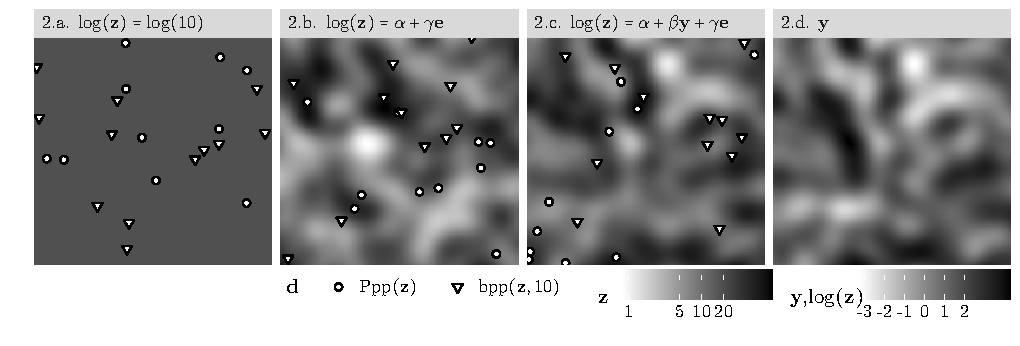
\includegraphics{fig/figure2.pdf}
    \vspace{-1cm}
    
    
    \footnotesize{
    
%
Sub-figures correspond to the  heatmap of a design variable $\desvar$ (Sub-figures 2.a, 2.b, 2.c) to the heatmap of $\signal$ (Sub-figure 2.d) and the plot of the samples (circle and triangle dots) drawn according to the two different designs. The values of $(\alpha, \beta ,\gamma)$ for each sub-figure are: 2.a: $(\log(10),0,0)$, 2.b:$(\log(10)-(0.5^2+0.3^2),0,\sqrt{0.5^2+0.3^2})$, 2.c: $(\log(10)-(0.5^2+0.3^2),0.5,0.3)$.}
%\end{mdframed}

\end{figure}

\begin{figure}[H]
%\begin{mdframed}
\caption{Joint and marginal densities of $\desvar$ and $\signal$}\label{fig:jointmarginaldensitiesYZ}
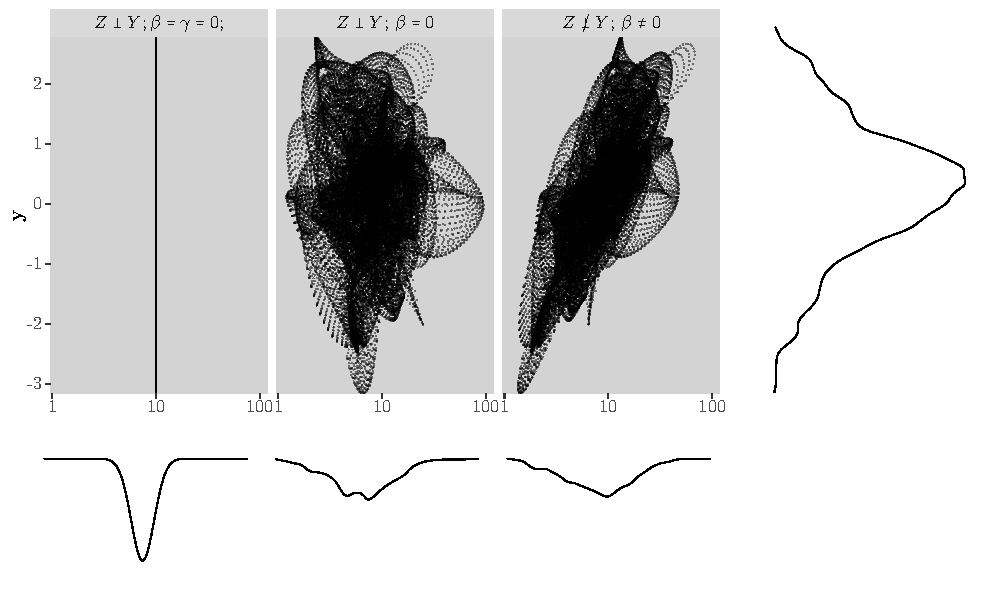
\includegraphics{fig/figure3.pdf}
\footnotesize{
 Each sub-figure contains the scatter plot of  $\left\{\left(\desvar[\position],\signal[\position]\right):\position\in\mathrm{Grid}\right\}$, where $\mathrm{Grid}$ is a regularly spaced grid of $\Pop$. The values of $(\alpha, \beta ,\gamma)$ for each Sub-figure are: 3.1: $(\log(10),0,0)$, 3.2:$(\log(10)-(0.5^2+0.3^2),0,\sqrt{0.5^2+0.3^2})$, 3.3: $(\log(10)-(0.5^2+0.3^2),0.5,0.3)$. The vertical axis corresponds to $\signal$, the vertical to $\desvar$. The marginal plots correspond to the density of $\desvar$ (right margin) and to the densities of $\signal$ (bottom margins).}
%\end{mdframed}
\end{figure}




\subsection{Observations}
The observation consists of the realisations of the random variables $\Sample$ and $\Signal[\Sample]$. 
%$(\Sample[\ell],\Signal[\Sample[\ell]])_{\ell\in\{1,\ldots,\Sampleindex}$
%Observations $(\Sample,\Signal[\Sample])=(\Sample[\ell],\Signal[\Sample[\ell]])_{\ell=1,\ldots,n}$ can be seen as a point process in $\Pop\times\SignalSpace$ and its intensity is defined as the Radon Nikodym derivative of $\Intensity_S$ with respect to the measure $\dominantU\otimes\dominantY$.


\section{Sample distribution}\label{sec:sampledistribution}

\subsection{Density ratio and weighted density.}
In this section, we derive the distribution of the observed values of the signal on the sample, (e.g. the distribution of $\Signal[\Sample]$) from  the distribution of the design variable conditionally $\Desvar$ to the signal $\Signal$ and the function that links the design to the design variable, or equivalently the distribution of the sample $\Sample$ conditionally to the Design variable $\Desvar$. To this end, we proceed step by step and resort to the Bayes formula. 



%{\color{red} Do we need the notation g ? the idea is that $g$ is the density for the sample. I am in favour of creating a command and call it $\pi$ instead.} 


\begin{definition}
For a random set $\Sampleindex$, 
define
$\rho_{\Sampleindex}(.\mid.)$ as any function that satisfies:

\begin{equation}
P^{(\Sample_\Sampleindex,\Signal[\Sample_\Sampleindex])}-\text{a.s}(\position,\signal),~\density_{\Signal[\position]\mid\Sample_\Sampleindex=\position}\left(\signal\right)=
    \density_{\Signal[\position]}\left(\signal\right)
    \rho_{\Sampleindex}\left(\position\mid  \signal\right)\label{eq:owijoj}
\end{equation}

\end{definition}


\begin{property}
%Let $\Sampleindex$ be a non random finite subset of $\mathbb{N}$, then
\begin{equation}
P^{(\Sample_\Sampleindex,\Signal[\Sample_\Sampleindex])}-\text{a.s}(\position,\signal),~~~
\rho_{\Sampleindex}\left(\position \mid \signal\right)=
    \frac{\density_{\Sample_\Sampleindex\mid \Signal[\position]}\left(\position|\signal\right)}{
         \density_{\Sample_\Sampleindex}\left(\position\right)}
\end{equation}


\end{property}

\begin{proof}
From the Bayes formula:
\begin{eqnarray}
\density_{\Signal[\position]\mid\Sample_\Sampleindex =\position }\left(\signal\right)
&=&(\density_{\Sample_\Sampleindex }(\position))^{-1}~\density_{\Signal[\position],\Sample_\Sampleindex }(\signal,\position)\\
&=&(\density_{\Sample_\Sampleindex }(\position))^{-1}~
\density_{\Sample_\Sampleindex \mid\Signal[\position]}(\position\mid \signal)~
\density_{\Signal[\position]}(\signal)\label{eq:oijoijsf}
\end{eqnarray}


So, combining Equations \eqref{eq:oijoijsf} and  \eqref{eq:owijoj}:
\begin{equation}
{\rho_{\Sampleindex}\left(\position \mid \signal\right)}
=(\density_{\Sample_\Sampleindex }(\position))^{-1}
~\density_{\Sample_\Sampleindex \mid\Signal[\position]}(\position\mid \signal)
\end{equation}
\end{proof}%

%Besides,
%\begin{equation}\label{eq:iurhiehgieurhg}
%\density_{\Sample_\Sampleindex }(\position)=
%\int \density_{\Sample_\Sampleindex \mid \Signal[\position]}(\position\mid \signal)~ \density_{\Signal[\position]}(\signal)~
%\derive \dominantY^{\otimes \Sampleindex}(\signal)
%\end{equation}

The density ratio $\densityratio$ can be derived from the distribution of $\Desvar$:

\begin{eqnarray}
\rho_{\Sampleindex}(\position\mid\signal)&=&\left({\int
         \density_{\Sample_\Sampleindex\mid \Desvar}\left(\position|\desvar\right)\derive P^{\Desvar}}\right)^{-1}{\int\density_{\Sample_\Sampleindex\mid \Desvar}(\position\mid\desvar)\derive P^{\Desvar\mid\Signal[\position]=\signal}(\desvar)}
\label{eq:oigjeogjio}\end{eqnarray}

However, there is not necessarily a close form for the integration of $\density_{\Sample_\Sampleindex\mid \Desvar}$ over $\desvar$, as shown in the two examples below.

\subsubsection*{Example (continued): Sample density ratios for $\Sample\sim \mathrm{Ppp}(\Desvar)$ and $\Sample\sim \mathrm{bpp}(\Desvar,n)$}
Conditionally on $\Signal[\position]=\signal$, $\Desvar$ is a log normal random process with distribution characterized by 
$E[\log(\Desvar[\position'])\mid \Signal[\position]=\signal]=\alpha+\beta(\mu+\Sigma_{\position',\position}\Sigma_{\position,\position}^{-1} (\signal-\mu))$ and 
$\mathrm{Var}[\log(\Desvar[\position'])\mid \Signal[\position]=\signal]=\gamma^2\provar_{x'}+\beta^2\left(\provar_{\position',\position'}-\provar_{\position',\position}\provar_{\position,\position}^{-1}\provar_{\position,\position'})\right)$.


\begin{proof}
See Appendix \ref{sec:A.owifjoeij}
\end{proof}



For $\position\in\Pop^{\{1,\ldots,\samplesize\}}$, when $\Sample\sim \mathrm{Ppp}(\Desvar)$,
\begin{equation}\density_{\Sample\mid W}(\position|\mathbf{w})=
\int\exp\left(-(\desvar.\dominantU)(\Pop)\right)(\samplesize!)^{-1}\left(\prod_{\ell=1}^\samplesize \desvar[\position(\ell)]\right)\derive
P^{\Desvar\mid W}(\desvar\mid \mathbf{w}),\label{eq:oijoijejods}
\end{equation}
and when $\Sample\sim \mathrm{bpp}(\Desvar,\samplesize)$,
\begin{equation}
\density_{\Sample\mid W}(\position|\mathbf{w})=
\int\left(-(\desvar.\dominantU)(\Pop)\right)^{-\samplesize}\left(\prod_{\ell=1}^\samplesize \desvar[\position(\ell)]\right)\derive
P^{\Desvar\mid W}(\desvar\mid \mathbf{w}).\label{eq:oijerogiql}
\end{equation}

A close form for \eqref{eq:oijerogiql} or \eqref{eq:oijoijejods} cannot be achieved when $W=\mathbf{w}$ is replaced by $\Signal[\position]=\signal$ (for the numerator of $\densityratio$) or $1=1$ (for the denominator).
And numerical approximation is numerically intensive.
However, we propose to use a very crude approximation:
$\intensityratio_{\Sampleindex}(\position\mid\signal)\approx\tilde{\intensityratio}_{\Sampleindex}(\position\mid\signal)$,
with 
$\tilde{\intensityratio}$  that is $P-a.s(\Sample_\Sampleindex,\Signal[\Sample_\Sampleindex])(\position,\signal)$- a.s. defined:

\begin{equation}\tilde{\intensityratio}_{\Sampleindex}(\position\mid\signal)=
\frac{
\mathrm{E}\left[\exp\left(\sum_{\ell\in\sampleindex}\beta \Signal[\position(\ell)]+\gamma \varepsilon[\position(\ell)]\right)\mid \Signal[\position]=\signal\right]}{
\mathrm{E}\left[\exp\left(\sum_{\ell\in\sampleindex}\beta \Signal[\position(\ell)]+\gamma \varepsilon[\position(\ell)]\right)\right]}\times
\frac{P(\Sampleindex\cap\{1,\ldots,N\})=\sampleindex\mid \Signal[\position]=\signal)}{P(L\cap\{1,\ldots,N\}=\sampleindex)}\label{eq:oeigjeoijioej}
\end{equation}
with $\sampleindex=\mathrm{domain}(\position)$.

A cruder approximation consists in neglecting the second factor in \eqref{eq:oeigjeoijioej}:

$$\tilde{\tilde{\intensityratio}}_{\Sampleindex}(\position\mid\signal)=
\frac{
\mathrm{E}\left[\exp\left(\sum_{\ell\in\sampleindex}\beta \Signal[\position(\ell)]+\gamma \varepsilon[\position(\ell)]\right)\mid \Signal[\position]=\signal\right]}{
\mathrm{E}\left[\exp\left(\sum_{\ell\in\sampleindex}\beta \Signal[\position(\ell)]+\gamma \varepsilon[\position(\ell)]\right)\right]}.$$

We obtain a close form for 
$\tilde{\tilde{\intensityratio}}$:

\begin{equation}
P^{(\Sample,\Signal[\Sample])}-\text{a.s.}(\position,\signal),
\tilde{\tilde{\intensityratio}}_{\{1,\ldots,N\}}(\position\mid\signal)=
\exp\left(\mathds{1}^T\beta(\signal-\mu\mathds{1})
-\frac12\mathds{1}^T\left(
\beta^2\provar_{\position,\position}
\right)\mathds{1}\right)\label{eq:kjeojmcxzmxz}
\end{equation}
\begin{proof}
See Appendix \ref{sec:ijojeorijgo}
\end{proof}


{\color{red}
This approximation is not satisfying: it does not depend on $\gamma$.
We need to work on that by investigating the distribution of the integral of a lognormal point process.
Cressie has some approximations that we could use.
}

\subsection{Distribution of $\Signal[\Sample]$}
The density of $\Signal[\Sample]$ with respect to $\dominantYbar$ is defined by
\begin{equation}\density_{\Sample,\Signal[\Sample]}(\position,\signal)=\rho_{\{1,\ldots,N\}}(\position\mid\signal)~\times~ \density_{\Signal[\position]}(\signal)~\times~\density_{\Sample}(\position).\label{eq:iuhsdewripeowi}\end{equation}

The "population distribution" is the distribution of $\Signal$, from which can be derived the distribution of $\Signal[\position]$ for any $n\in\mathbb{N}$, and any $\position\in \Pop^n$. The distribution of $\Signal$ is defined by all its finite dimensional distributions.
The "sample distribution" is the distribution of an imaginary process $\Signal^\star$ such that its finite-dimensional distributions $\density_\Signal^\star[\position]$, for any $\position \in\toPop$ are given by
$$\density_\Signal^\star[\position]=
 \rho_{\{1,\ldots,N\}}(\position\mid\signal)~\times~ \density_{\Signal[\position]}.$$

Generalising \cite{pfefferman_1992}, the selection is non informative when $P^{\Signal[\Sample],\Sample}-\text{a.s.}(\signal,\position)$, $\rho(\position,\signal)=1$. In this case, we consider that the sample distribution corresponds to the population distribution.



This general definition of a sample process by opposition to the population process allows to define the sample counterpart of different characteristics of the population distribution as for example the intensity and the covariogram.

Although we gave a theoretical definition of $\rho$, as in practice a close form may be difficult to obtain, one can also define the approximated finite dimensional densities of $\Signal^\star$ 
$$\tilde{\tilde{\density}}_{\Signal^\star[\position]}(\signal)=\tilde{\tilde{\density}}_{\Signal[\Sample]\mid\Sample}(\signal\mid\position)=
\tilde{\tilde{\densityratio}}_{\{1,\ldots,\Samplesize\}}(\position\mid\signal)\density_{\Signal[\position]}(\signal).$$

\subsection{Sample Intensity}

\subsection{Sample Variogram}
Define the sample semi variogram for exchangeable designs as 

$$\Semivariogram^\star(h)=\frac12~\E\left[\left(\Signal[\Sample[1]]-\Signal[\Sample[2]]\right)^2\mid \Sample[2]-\Sample[1]=h\right].$$

\begin{property}[Relationship between $\Semivariogram$, $\Semivariogram^\star$ and $\rho$]
$$\Semivariogram(h)^\star=\frac12\int_{\Pop^{\{1,2\}}} \left[\int_{\range{\Signal}^{\{1,2\}}} (\signal(2)-\signal(1))^2~ \density_{\Signal[\position]}(\signal)~
\intensityratio_{\{1,2\}}(\position,\signal)~
\derive\dominantY^{\otimes 2}(\signal)
\right] \derive(\dominantU^{\otimes\{1, 2\}})^{X\mid X[2]-X[1]=h}(\position)$$


\end{property}

\begin{proof}

\begin{eqnarray*}
\lefteqn{\E\left[\left(\Signal[\position(2)]-\Signal[\position(1)]\right)^2\mid \Sample_{\{1,2\}}=\position\right]}\\
&=&\int_{\range{\Signal}^2} (\signal(2)-\signal(1))^2~
\density_{\Signal[\position]\mid S_{\{1,2\}}}(\signal\mid \position)~
\derive\dominantY^{\otimes\{1, 2\}}(\signal) \\
&=&\int_{\range{\Signal}^2} (\signal(2)-\signal(1))^2~
\rho_{\{1,2\}}(\position,\signal)~ \density_{\Signal[\position]}(\signal)~
\derive\dominantY^{\otimes\{1, 2\}}(\signal) \\
\end{eqnarray*}


\end{proof}

%\subsubsection*{Example (continued)}
%
%Define the approximated sample variogram by replacing $\rho_{\{1,2\}}$ by $\tilde{\rho_{\{1,2\}}}$ in the expression of the sample variogram:
%$$\tilde\Semivariogram(h)^\star=
%\Semivariogram(h)
%\int\left(\int
%(\signal'(2)-\signal'(1))^2~ \frac{\mathrm{e}^{-\frac{(\signal')_1^2+(\signal')_2^2}{2}}}{2\pi}~
%\derive\dominantY^{\otimes \{1,2\}}(\signal')\right). 
%$$
%
%\begin{proof}
%See Appendix \ref{labelnotdoneyet}
%\end{proof}





\section{Estimation} \label{sec:estimation}

\subsection{Naive non parametric estimation : the case of the variogram}
%\subsubsection{Naive estimators and their properties in the non informative selection case}
With the term \emph{naive estimation} we refer to the situation where the estimator does not take into account the mechanism selection. Therefore, in case of informative sampling, the estimator could suffer from selection bias.
A common approach to achieve a valid variogram estimator is composed by \emph{estimation} and \emph{fitting} of the variogram. In the former, an estimate of the variogram is obtained, while the latter phase is necessary since the estimators used in the first phase are usually not conditionally negative-definite.

Under the assumption of constant-mean, an estimator based on the method of moments is \citep{matheron1962traite}
\begin{equation*} \label{eq:variogram_hat}
2\hat{\gamma}\left(h\right)=\frac{1}{|N\left(h\right)|}\sum_{(\ell_1,\ell_2)\in N\left(h\right)}{\left(\Signal\left[\Sample[\ell_1]\right]-\Signal\left[\Sample[\ell_2]\right]\right)^{2}},\forall h\in\mathbb{R}^{d}
\end{equation*}

where $N\left(h\right)=\left\{\left(\ell_1,\ell_2\right)\in\{1,\ldots,\Samplesize\}^2:\Sample[\ell_1]-\Sample[\ell_2]=h\right\}$ and $|N\left(h\right)|$ is the number of distinct pairs in $N\left(h\right)$. 

\begin{property}
$E[N(h)\hat{\Semivariogram}(h)]=\Semivariogram(h)$
\end{property}


When data are irregularly spaced in $\mathbb{R}^{d}$, we can use
\begin{equation} \label{eq:variogram_hat1}
2\hat{\gamma}_{s}\left(h\left(l\right)\right)=\mathrm{average}\lbrace\left(\Signal\left[\Sample[\ell_1]\right]-\Signal\left[\Sample[\ell_2]\right]\right)^{2}:%\left(\Sample[\ell_1], \Sample[\ell_2]\right)\in N\left(h\right);
\|\Sample[\ell_1]-\Sample[\ell_2]\|\in[h\mp \alpha]\rbrace,
\end{equation}
where the tolerance $\alpha$ is a positive number.
%the region $T\left(h\left(l\right)\right)$ is a specified tolerance region in $\mathbb{R}^{d}$ around $h\left(l\right)$ $l=1,\dots,K$ {\color{red} Check variable $l$}.

%A robust version of \eqref{eq:variogram_hat} is given by \citep{cressie1980robust}
%\begin{equation} \label{eq:variogram_hat_robust}
%2\hat{\gamma}_{r}\left(h\right)=\Bigg\lbrace\frac{1}{|N\left(h\right)|}\sum_{N\left(h\right)}{|\Signal\left[\Sample[\ell_1]\right]-\Signal\left[\Sample[\ell_2]\right]|}^{1/2}\Bigg\rbrace ^{4}
%/ \left(0.457 + 0.494/|N\left(h\right)|\right)
%\end{equation} 
%and corresponding smoothed version
%\begin{equation}
%2\hat{\gamma}_{rs}=\left[med\lbrace|\Signal\left[\Sample[\ell_1]\right]-\Signal\left[\Sample[\ell_2]\right]|^{1/2}:\left(\Sample[\ell_1], \Sample[\ell_2]\right)\in N\left(h\right);h\in T\left(h\left(l\right)\right)\rbrace\right]^{4}/B\left(h\right)
%\end{equation}
%where $med$ is the median of the sequence and $B\left(h\right)$ is a correction-term for bias (asymptotically $B\left(h\right)=0.457$).

%A non-parametric approach to variogram estimation can be achieved by the use of kernel estimator
%\begin{equation}
%2\hat{\gamma}\left(h\right)=\frac{\sum_{i}\sum_{j}{w_{ij}\left(h\right)\left(\Signal\left[\Sample[\ell_1]\right]-\Signal\left[\Sample[\ell_2]\right]\right)^{2}}}{\sum_{i}\sum_{j}{w_{ij}\left(h\right)}}
%\end{equation}
%where $w_{ij}=K\left(\frac{h-||\Sample[\ell_1] - \Sample[\ell_2]||}{g}\right)$, $K$ is a symmetric, zero-mean (bounded) and $g$ is a positive number called bandwith.

%{\color{red}FP: I do not know if the following makes sense.} To sum up, we can write a general estimator form for the \emph{naive estimated variogram}
%\begin{equation} \label{eq:g_hat}
    %\hat{G}(h)=\sum_{ij\in\Sample}{\beta_{ij}(h)(\Signal\left[\Sample[\ell_1]\right]-\Signal\left[\Sample[\ell_2]\right])(\Signal\left[\Sample[\ell_1]\right]-\Signal\left[\Sample[\ell_2]\right])^{T}}
%\end{equation}
%where the term $\beta_{i,j}$ is a mapping that depends on the particular estimator used (and sample selected).

Once the estimated variogram is obtained (or \emph{empirical}), a model is fitted to it in order to achieve a valid variogram. At this stage, we are searching for a valid variogram ``closest'' to the empirical one, and typically we look into a subset of valid variograms $P=\lbrace2\gamma:2\gamma\left(\cdot\right)=2\gamma\left(\cdot;\parampop\right);\parampop\in\parampop\rbrace$. The best element of $P$ can be searched through several good-of-fitness criteria, such as maximum likelihood estimator or Least Squares method.

%Maximum Likelihood estimator relies heavily on Gaussian assumption, while Least Squares method requires few assumption about $Y\left(\position\right)$.
%The LS minimizing problem can be written as 
%\begin{equation*}
%min\lbrace\left(2\tilde{\gamma}-2\gamma\left(\parampop\right)\right)^{T}W^{-1}\left(\tilde{\gamma}-\gamma\left(\parampop\right)\right)
%\end{equation*}
%where $2\tilde{\gamma}$ is the empirical variogram, $2\gamma\left(\parampop\right)$ is a valid model variogram with the exact form known except the parameter $\parampop$, and $W$ is a weight matrix. If $W$ is an identity matrix, Ordinary Least Square criterion is employed; in case of $W=V$, with $V$ variance-covariance matrix, we have Generalized Least Square criterion, and if $V$ is diagonal, Weighted Least Square criterion is achieved.

In order to investigate the behaviour of the naive estimation, we carried out a Monte Carlo simulation. We simulated one replication of the same isotropic Gaussian process considered in the Example 1, that is $\Signal:\Omega\to(\Pop=[0,1]^2\to\mathbb{R})$, with $\forall \position\in\Pop$, $\mathrm{\mu}[\position]=0$ and with a Gaussian Covariogram with parameters $\parampop_1=5$, $\parampop_2=0.1$. Samples were selected by means of $\mathrm{bpp}(1, 100)$, $\mathrm{bpp}(\desvar_{1}, 100)$, and $\mathrm{bpp}(\desvar_{2}, 100)$, where  $\mathbf{\desvar}_{1}$ is generated with parameters $(\log(10)-(0.4^2+0.3^2),0,\sqrt{0.4^2+0.3^2})$, and $\mathbf{\desvar}_{2}$ is generated with parameters  $(\log(10)-(0.4^2+0.3^2),0.4,0.3)$, as in the Example 2.
The $\mathrm{bpp}(1, \samplesize)$ is by definition a non-informative sampling mechanism, while the $\mathrm{bpp}(\desvar, \samplesize)$ could introduce bias when the variable $\desvar$ is correlated with the signal $\signal$, as explained in the previous Sections. Note that $\desvar_{1}$ was generated independently from $\signal$ while $\desvar_{2}$ was generated dependently from $\signal$. Indeed, $\mathrm{cor}(\signal, \desvar_{1})\approx -0.08$ and $\mathrm{cor}(\signal, \desvar_{2})\approx 0.75$, where $\mathrm{cor}$ indicates the correlation between the two variables. For each sampling mechanism, $M=1,000$ samples were selected, and variograms estimated by the method of moments and fitted by the Weighted Least Square criterion. These estimated variograms are compared to the variogram obtained by using all the population values, which we call \emph{population variogram}. In the first row of Figure \ref{fig:sim_naive_est}, we compare the averages of the densities obtained by samples selected by means of the three different selection mechanisms. We note that when $\mathrm{bpp}(\desvar_{2}, 100)$ is employed, the average density is different from the \emph{population density}. In the second row of Figure \ref{fig:sim_naive_est}, we compare the expected value of the variograms obtained by the replications to the population variogram. The simulation shows that when the samples are selected by means of $\mathrm{bpp}(1, 100)$ and $\mathrm{bpp}(\desvar_{1}, 100)$, the Monte Carlo expected value of the sample variogram (indicated by the dotted line) is close to the population variogram (indicated by continuous line), while when the samples are selected by means of $\mathrm{bpp}(\desvar_{2}, 100)$, the Monte Carlo expected value of the sample variogram (indicated by the dotted line) is  different from the population variogram (continuous line). Therefore, bias is introduced by the selection mechanism.

\begin{figure}[H]
\caption{Naive estimation of the variogram. In the first row, average densities (dotted lines) are compared with the population density (continuous line). In the second row, expected values of the variogram (dotted lines) are compared with population variogram (continuous line).}
\centering
\includegraphics[width=0.7\textwidth]{fig/fig4.png}
\label{fig:sim_naive_est}
\end{figure}

%\begin{figure}[H]
%\caption{Relative Mean Squared Error to $\mathrm{bpp}(1, 100)$ of the variogram estimation}
%\label{fig:naive_est2}
%\centering
%\includegraphics[width=0.6\textwidth]{fig/rmse.png}
%\end{figure}


\subsection{Maximum likelihood estimation}
%In particular, with ML we assume that the data $\Signal$ are multivariate Gaussian $(\textbf{X}\boldsymbol{\beta},{\color{red}\provar_{\position,\position^{'};\parampop}}$. The negative loglikelihood is {\color{red} FP: notation needs to be checked.} 
%{\color{red} DB: Can we just take the model with beta=0, Gaussian covariogram, $\parampop$ parameter of the covariogram (scale $\parampop_2$, and $\parampop_!=\sigma$).} 

%\begin{equation} \label{fit:ML}
%\likelihood\left(\boldsymbol{\beta},\parampop\right)=\left(n/2\right)\log{\left(2\pi\right)}+\left(1/2\right)\log{|\provar_{\position,\position^{'};\parampop}|}
%+\left(1/2\right)\left(\Signal-\textbf{X}\boldsymbol{\beta}\right)^{T}\provar_{\position,\position_{'};\parampop}^{-1}\left(\Signal-\textbf{X}\boldsymbol{\beta}\right)
%\end{equation}
%with estimators $\boldsymbol{\hat{\beta}}$ and $\hat{\parampop}$ satisfying $L\left(\boldsymbol{\hat{\beta}},\hat{\parampop}\right)=\inf{\lbrace L\left(\beta,\parampop\right):\boldsymbol{\beta}\in\mathbb{R}^{{\color{red}q}},\parampop\in\parampop\rbrace}$.

%\begin{equation} \label{fit:ML}
%\likelihood\left(\parampop\right)=\left(n/2\right)\log{\left(2\pi\right)}+\left(1/2\right)\log{|\provar_{\position,\position^{'};\parampop}|}
%+\left(1/2\right)\left(\Signal\right)^{T}\provar_{\position,\position_{'};\parampop}^{-1}\left(\Signal\right)
%\end{equation}
%with estimators $\hat{\parampop}$ satisfying $L(\hat{\parampop})=\inf{\lbrace L\left(\parampop\right):\parampop\in\parampop\rbrace}$.

Here we briefly present a possible solution that take into account the informativeness  of the sample. The proposal is based on the maximum likelihood estimation. In particular, in our setup, the loglikelihood of $\Signal[\position]$ is given by 

\begin{eqnarray} \label{Lnaive}
\likelihood_{\Signal[\position]}\left(\parampop;\signal\right)&=&\log(\density_{\Signal[\position]}(\signal;\parampop))\\&=&
\frac12\log{|\provar_{\position,\position^{'};\parampop}|}
+\frac12(\Signal[\Sample])^{\mathrm{T}}\provar_{\position,\position_{'};\parampop}^{-1}\Signal[\Sample]
\end{eqnarray}

and the naive estimator maximizes \eqref{Lnaive}. Indeed, this maximization ignores the selection mechanism. 

In order to take into account the informativeness of the sample, the \emph{full loglikelihood} should be used, which is composed by three factors: the density ratio, $\densityratio_{\Sample}(\position\mid\signal)$, the distribution of $\Signal$, $\density_{\Signal[\position]}(\signal)$, and the distribution of the sample, $\density_\Sample(\position)$. Therefore the loglikelihood is 

\begin{eqnarray} \label{fit:ML2}
\likelihood_{\Sample,\Signal[\Sample],\Samplesize}\left(\parampop,\paramnuisance;\position,\signal,\samplesize\right)&=&\log\left(\densityratio_{\Sample}(\position\mid\signal;\parampop,\paramnuisance)\right)+\log(\density_{\Signal[\position]}(\signal;\parampop))+\log\left(\density_\Sample(\position;\parampop,\paramnuisance)\right)
\end{eqnarray}

%{\color{red} Discuss here about what we do about $\density_\Sample(\position)$. Why we ignore it, although it may still contain information about $\theta$ and $\xi$, link to the debate about estimation in presence of nuisane parameters, reference to my draft paper and the approaches. Marginalisation or conditioning}


%REML estimators are obtained by applying maximum likelihood over error contrasts instead of the original data. %In the context of variogram estimation, the idea is to apply the likelihood over $\textbf{W}=\left(\Signal\left(1\right)-\Signal\left(2\right),\Signal\left(2\right)-\Signal\left(3\right),\dots,\Signal\left(n-1\right)-\Signal\left(n\right)\right)$
%Defining a vector of $n-\text{rank}\left(\Position\right)$ linearly independent (error) contrasts as $R=A^{T}\Signal$, where $A$ is an $\left(n-1\right)\times n$ matrix with elements
%\[
%a_{ij}=
%\begin{cases}
%1 &\text{for }i=j,j=1,\dots,n-1, \\
%-1&\text{for }i=j+1,j=1,\dots,n-1,\\
%0 &\text{elsewhere.}
%\end{cases}
%\]
%we have that $R\sim N\left(\textbf{0},A^{T}\provar_{\position,\position^{'};\parampop}A\right)$, which does not depend on $\boldsymbol{\beta}$. Moreover, if $A$ satisfies $AA^{T}=I-\Position\left(\Position^{T}\Position\right)^{-1}\Position^{T}$ and $A^{T}A=I$, we then have the following negative likelihood
%\begin{align*}
%L_{R}\left(\parampop\right)&=\left(\left(n-q\right)/2\right)\log{\left(2\pi\right)}-\left(1/2\right)\log{|\Position^{T}\Position|}+\left(1/2\right)\log{|\provar_{\position,\position^{'};\parampop}|}\\&+\left(1/2\right)\log{|\Position^{T}\provar_{\position,\position^{'};\parampop}^{-1}\Position |}+\left(1/2\right)\Signal^{T}\Pi\left(\parampop\right)\Signal
%\end{align*}
%where $\Pi\left(\parampop\right)=\provar_{\position,\position^{'};\parampop}^{-1}-\provar_{\position,\position^{'};\parampop}^{-1}\Position\left(\Position^{T}\provar_{\position,\position^{'};\parampop}^{-1}\Position\right)^{-1}\Position^{T}\provar_{\position,\position^{'};\parampop}^{-1}$ . Therefore, the REML estimate of $\parampop$ is obtained by minimizing $L_{R}\left(\parampop\right)$ over $\parampop$.




%Exact finite-sample distribution theory for estimators and corresponding variance estimators are available only in special circumstances (e.g. Jensen 1988). Therefore, simulations or approximation theory need to be employed in order to deal with intractable distribution theory. \cite{zimmerman1991comparison} presented a Monte Carlo comparison of different estimators, when two intrinsically stationary isotropic Gaussian random processes in $\mathbb{R}^{2}$ and various sampling intensities are taken into account. With regard to the MLE, different Authors agree that such approach can suffer from bias. \cite{warnes1987problems} illustrate potential problems by simulations of some simple spatial process, and \cite{mardia1989multimodality} indicate that these problems are caused by likelihoods not twice differentiable in $\parampop$. Moreover, a general conclusion that emerges from a set of several works based on simulations (Haining 1978c, Mardia and Meshall 1984, Swallow and Monahan 1984, Haining et al 1989, Zimmerman and Zimmerman 1991) is that the bias of MLE tends to be negative when the spatial dependence is positive, especially for small sample size. %{\color{red}and asymptotic variances of small-scale variation parameters are good approximation to exact variances only when the spatial dependence is weak.}

%For approximation theory, Cressie talks about two type of asymptotic theories {\color{red} pp }. \emph{Infill asympotics} refers to the the possibility to increase the sample size to infinity while the finite domain $D$ is kept fixed, whereas \emph{increase-domain asymptotics} refers to the situation where we take more units by means of increase the domain $D$. 

%Taken as it is from Cressie book (Section 7.3.1): when making inference on a random field $\lbrace Z(s):s\in D\rbrace$ from data $Z=(Z(s_{1},Z(s_{2}),\dots,Z(s_{n}))$, exact distribution theory of estimators, predictors, test statistics, and so on, is rarely available. Asymptotic distribution theory is the natural place to run for approximations, although, spatially, there are number of ways $n$ might tend to infinity.

%The \emph{naive estimated variogram} is 
%\begin{equation} \label{eq:g_hat}
    %\hat{G}(h)=\sum_{ij\in\Sample}{\beta_{ij}(h)(\Signal(\position_{i})-\Signal(\position_{j}))(\Signal(\position_{i})-Y(\position_{j}))^{T}}
%\end{equation}
%In equation \eqref{eq:g_hat}, the term $\beta_{i,j}$ is a mapping that may depend on the sample selected.
%Below we give possible definitions of $\beta_{i,j}$:
%\begin{equation}
    %\beta(\position_1,\position_2,h)=
    %\left|\begin{array}{l}
    %1 \text{ if } |\position_1-\position_2|=h, 0 \text{ otherwise}\\
    %\paramnuisance(\frac{|\position_{i}-\position_{j}|-h}{\alpha})
    %\end{array}\right.
%\end{equation},
%For binned estimation, a finite partition $(B_1,\ldots,B_n)$ of $\mathbb{R}^+$ is given as well as an element $h_k$ of each element $B_k$ of the partition. 
%Then the covariogram is first estimated for each $h_k$, as 
%...
%Then a covariogram is fitted 
%...
%In the following, we will not consider binned estimation.
%where {\color{red} $\paramnuisance$ is ..., and the bins $\mathrm{bin}_h=\left\{(i,j)\in\Sample^2\mid \left|\position_i-\position_j\right|\in [a_h,b_h)\right\}$}

%\subsection{Properties of the sample in the general case (including informative)}



 %Naive estimation of the population covariogram:
 %$E[naive~Covariogram]\neq$ pop cov,
 %$E[naive~Covariogram]=$ sample theoretical cov, 
 %with illustrative figures.




%\subsection{Parametric estimation}


\section{Prediction} \label{sec:prediction}
%The variogram is a useful tool in order to quantify the spatial dependence in the data/process. Therefore, use of it in the inferential process has been investigated. We focus on the \emph{kriging} {\color{red} \citep{matheron1962traite}}, which is a minimum mean squared error method of spatial prediction that takes full advantage of the variogram. In fact, the kriging estimator incorporates the covariance structure of the $\Signal$ into the weights. In particular, the weights are based on the covariance among sample points and the covariance between sample points and predicted points. Note that this does not happen in distance-based method, where the weights depend only on the location of the points.

%{\color{red} In the follow just some notes about ordinary kriging, it needs to be completed/reviewed}
%\emph{Ordinary kriging} assumes following model
%\begin{equation}
%\Signal\left(\position\right)=\mu+\delta\left(\position\right)
%\end{equation}
%where $\position\in\mathbb{R}^{d}$, $\mu\in\mathbb{R}$, and $\mu$ unknown, and following predictor
%\begin{equation}
%P\left(\Signal,\Position\right)=\sum_{i=1}^{n}{\lambda_{i}\Signal\left(\position\right)}
%\end{equation}
%The weights $\lambda_{i}$s are computed such that the estimator is unbiased and the variance is minimized. {\color{red} Needs more here}


%\subsection{Naive prediction and prediction that accounts for informative selection}

The following property provides the formula for the predictive distribution of $\Signal[\position']$ when $\Sample,\Signal[\Sample]=\position,\signal$ is observed.

\begin{property}
The probability density function of $\Signal[\position']$ conditionally on $(\Sample,\Signal[\Sample] =(\position,\signal)$ is given, for $\position'\in\toPop,
\signal'\in\SignalSpace^{\{1,\ldots,\size(\position')\}}$ by:
\begin{equation}
P^{\Sample,\Signal[\Sample]}-\text{a.s.}(\sample,\signal),~ \density_{\Signal[\position']\mid\Sample,\Signal[\Sample]}(\signal'\mid\position,\signal)
=\frac{
\density_{\Sample\mid\Signal[\position]=\signal,\Signal[\position']}(\position\mid\signal,\signal')
}{
\density_{\Sample\mid\Signal[\position]}(\position\mid\signal)
}~\times~\density_{\Signal[\position']\mid\Signal[\position]}(\signal'\mid\signal)
\end{equation}
\end{property}
\begin{equation*}
\frac{
\density_{\Sample\mid\Signal[\position]=\signal,\Signal[\position']}(\position\mid\signal,\signal')
}{
\density_{\Sample\mid\Signal[\position]}(\position\mid\signal)
}=
\frac{
\int 
\frac{\exp\left(-\paramnuisance_1(\sum_{\ell=1}^2\signal(\ell)-\paramnuisance_2(\sum_{\ell=1}^{\samplesize'}\varepsilon[\position(\ell)])\right)}{\left(\int \exp\left(-\paramnuisance_1\Signal[\position']-\paramnuisance_2\varepsilon[\position']\right)\derive\nu(\position')\right)^{\samplesize'}}\derive P^{\Signal,\varepsilon\mid \Signal[\position]=\signal,\Signal[\position']=\signal'} 
}{
\int 
\frac{\exp\left(-\paramnuisance_1(\sum_{\ell=1}^{\samplesize'}\Signal[\position(\ell)]-\paramnuisance_2(\sum_{\ell=1}^{\samplesize'}\varepsilon[\position(\ell)])\right)}{\left(\int \exp\left(-\paramnuisance_1\Signal[\position']-\paramnuisance_2\varepsilon[\position']\right)\derive\nu(\position')\right)^{\samplesize'}}\derive P^{\Signal,\varepsilon\mid \Signal[\position]=\signal} \phantom{11111} 
}.
\end{equation*}
\section{Conclusions} \label{sec:conclusions}
We have extended the notions of informative selection, population and sample distributions defined by \cite{pfefferman_1992} to a situation where a spatial process is assumed to have generated the whole population. In particular, a Gaussian random field and two point processes that represent the selection mechanism have been considered. An analysis of the naive estimation of the variogram have been performed, and simulation shows that selection bias is introduced when there is dependence between the superpopulation model and the mechanism selection. Finally, we briefly discussed a possible solution in order to correct the naive estimation in presence of informative selection. This solution is based on the use of the maximum likelihood. Future research will be dedicated to a proper development of such proposal.


\section*{Acknowledgements}
We developed an R package that allows to reproduce all the simulation results see \cite{gitSpatialInformativeSelection}. Francesco Pantalone's work was partially funded by the \emph{``International Graduate Research Fellowships''} at Joint Program in Survey Methodology, University of Maryland, College Park, USA.
\appendix


\newpage
\section{Algebra for the example}

\subsection{Distribution of  $\Desvar$ conditionally on  $\Signal[\position]=\signal$}\label{sec:A.owifjoeij}
Under the condition of the paper example, conditionally on $\Signal[\position]=\signal$, the process $(\alpha+\beta\Signal+\gamma\varepsilon)$ is a Gaussian Process characterised by
$\mathrm{E}\left[(\alpha+\beta\Signal+\gamma\varepsilon)[\position']\right]=\alpha+\beta(\mu+\Sigma_{\position',\position}\Sigma_{\position,\position}^{-1} (\signal-\mu))$ and  $\mathrm{Var}\left[(\alpha+\beta\Signal+\gamma\varepsilon)[\position']\right]=\gamma^2\provar^\varepsilon_{\position',\position'}+\beta^2(\provar_{\position',\position'}-\provar_{\position',\position}\provar_{\position,\position}^{-1}\provar_{\position,\position'})$, and consequently, conditionally on $\Signal[\position]=\signal$, $\Desvar=\exp(\alpha+\beta\Signal+\gamma\varepsilon)$ is a lognormal spatial process.

%
%
%\begin{eqnarray*}
%\lefteqn{W[\position'_{1},\ldots,\position'_{m}]\mid\Signal[\position_{1},\dots,\position_{n}]=
%    \signal}\\&\sim&
%   P^{\alpha+\gamma\varepsilon[\position']}
%   \ast 
%    P^{\beta\Signal[\position']\mid\Signal[\position]=
%    \signal}\\&&=\ 
%   \mathrm{Normal}(\alpha+\beta(\mu+\Sigma_{\position',\position}\Sigma_{\position,\position}^{-1} (\signal-\mu)),
%\gamma^2\provar^\varepsilon_{\position',\position'}+\beta^2(\provar_{\position',\position'}-\provar_{\position',\position}\provar_{\position,\position}^{-1}\provar_{\position,\position'}))
%    \end{eqnarray*}

\begin{proof}

\begin{eqnarray}\lefteqn{\begin{bmatrix}
\Signal[\position']\\
\Signal[\position]
\end{bmatrix}\sim\mathrm{Normal}\left(\mu,\begin{bmatrix}\provar_{\position',\position'}&\provar_{\position',\position}\\
\provar_{\position,\position'}&
\provar_{\position,\position}
\end{bmatrix}\right)}\\
&\Rightarrow&
\left[
\left.\Signal[\position']
\right|
\Signal[\position]=\signal
\right]
\sim\mathrm{Normal}\left(\mu+\Sigma_{\position',\position}\Sigma_{\position,\position}^{-1} (\signal-\mu),\Sigma_{\position',\position'}-\Sigma_{\position',\position}\Sigma_{\position,\position}^{-1}\Sigma_{\position,\position'}\right)\label{eq:hfqopio}\end{eqnarray}

The independence of $\varepsilon$ and $\Signal$ implies that:
\begin{equation}\label{eq:iushfisduhsd}\left[\left.
\varepsilon[\position']
\right|
\Signal[\position]=\signal
\right]\sim\mathrm{Normal}\left(\mu_\varepsilon,\provar_{\position',\position';\varepsilon}\right),\end{equation} and that the vector obtained by stacking $\Signal[\position]$, $
\Signal[\position']$, and $\varepsilon[\position']$ is normal. 
By combining \eqref{eq:iushfisduhsd} and \eqref{eq:hfqopio} we obtain that:

$$\left[\left.\begin{bmatrix}
\Signal[\position']\\
\varepsilon[\position']
\end{bmatrix}\right|
\Signal[\position]=\signal
\right]\sim\mathrm{Normal}\left(\begin{bmatrix}\mu+\Sigma_{\position',\position}\Sigma_{\position,\position}^{-1} (\signal-\mu)\\0\end{bmatrix},
\begin{bmatrix}\Sigma_{\position',\position'}-\Sigma_{\position',\position}\Sigma_{\position,\position}^{-1}\Sigma_{\position,\position'}&0\\0&\provar_{\position',\position';\varepsilon}\end{bmatrix}\right).$$

We obtain the moments of $Z[\position']=\gamma
\varepsilon[\position']+\alpha+\beta
\Signal[\position']$ conditionally on $\Signal[\position]=\signal$:
$$\mathrm{E}\left[\alpha+\beta
\Signal[\position']+\gamma
\varepsilon[\position']|
\Signal[\position]=\signal\right]
=\alpha+\beta(\mu+\Sigma_{\position',\position}\Sigma_{\position,\position}^{-1} (\signal-\mu)),$$
and 
$$\mathrm{Var}\left[\alpha+\beta
\Signal[\position']+\gamma
\varepsilon\left[\position'\right]|
\Signal[\position]=\signal\right]
=\gamma^2\provar_{\position',\position';\varepsilon}+\beta^2\left(\provar_{\position',\position'}-\provar_{\position',\position}\provar_{\position,\position}^{-1}\provar_{\position,\position'})\right).$$
\end{proof}



\subsection{Proof of Equation \eqref{eq:kjeojmcxzmxz}}
\label{sec:ijojeorijgo}

The first moment of a lognormal distribution of parameters $m$ and $s^2$ is $exp(m+s^2/2)$, so 
\begin{eqnarray*}
\lefteqn{
\mathrm{E}\left[\exp\left(\sum_{\ell\in\sampleindex'}\beta \Signal[\position'(\ell)]+\gamma \varepsilon[\position'(\ell)]\right)\mid \Signal[\position]=\signal\right]}
\\&=&
\exp\left(\mathds{1}^T\beta(\mu\mathds{1}+\Sigma_{\position',\position}\Sigma_{\position,\position}^{-1} (\signal-\mu\mathds{1}))+
\frac12\mathds{1}^T\left(
\gamma^2\provar_{x'}+\beta^2\left(\provar_{\position',\position'}-\provar_{\position',\position}\provar_{\position,\position}^{-1}\provar_{\position,\position'})\right)
\right)\mathds{1}\right)
\end{eqnarray*}
which simplifies when $\position'=\position$ to 

\begin{eqnarray*}
\mathrm{E}\left[\exp\left(\sum_{\ell\in\sampleindex}\beta \Signal[\position(\ell)]+\gamma \varepsilon[\position(\ell)]\right)\mid \Signal[\position]=\signal\right]&=&
\exp\left(\mathds{1}^T\beta\signal+
\frac12\mathds{1}^T\left(
\gamma^2\provar_{\position,\position;\varepsilon}
\right)\mathds{1}\right)
\end{eqnarray*}

and when $\position=\mathbf{0}$:
\begin{eqnarray*}
\mathrm{E}\left[\exp\left(\sum_{\ell\in\sampleindex'}\beta \Signal[\position'(\ell)]+\gamma \varepsilon[\position'(\ell)]\right)\right]
&=&
\exp\left(\mathds{1}^T\beta\mu\mathds{1}+
\frac12\mathds{1}^T\left(
\gamma^2\provar_{\position',\position',\varepsilon}+\beta^2\left(\provar_{\position',\position'})\right)
\right)\mathds{1}\right)
\end{eqnarray*}

So:

\begin{equation}
\tilde{\tilde{\intensityratio}}_{\{1,\ldots,N\}}(\position\mid\signal)=
\exp\left(\mathds{1}^T\beta(\signal-\mu\mathds{1})+
\frac12\mathds{1}^T\left(
-\beta^2\left(\provar_{\position,\position})\right)
\right)\mathds{1}\right)\label{eq:kjeojmcxzmxz}
\end{equation}



\subsection{Algebra for the denominator of $\rho$}

The denominator of $\rho$ requires the computation of $\int_{U}\Sigma_{\position',\position}~d\dominantU$, which is itself a function of
$\int_{U}\Covariogram(\position'-\position_j)d\dominantU\left(\position'\right)$


For $\position=(\position_1,\position_2)$, such that $\|\position_1-\position_2\|=h$, we have the following:

\begin{eqnarray*}
\Sigma_{\position,\position}&=&
    \begin{bmatrix}\Covariogram(0)&\Covariogram(h)\\\Covariogram(h)&\Covariogram(0)\end{bmatrix}\\
\Sigma_{\position,\position}^{-1}&=&
    (\Covariogram(0)^2-\Covariogram(h)^2)^{-1}\begin{bmatrix}\Covariogram(0)&-\Covariogram(h)\\-\Covariogram(h)&\Covariogram(0)\end{bmatrix}\\
\Sigma_{\position',\position}\Sigma_{\position,\position}^{-1}
    &=&(\Covariogram(0)^2-\Covariogram(h)^2)^{-1}
        \begin{bmatrix}\Covariogram(\position'-\position_1)&\Covariogram(\position'-\position_2)\end{bmatrix}\begin{bmatrix}\Covariogram(0)&-\Covariogram(h)\\-\Covariogram(h)&\Covariogram(0)\end{bmatrix}\\
    &=&\frac{\begin{bmatrix}
        \Covariogram(0)\Covariogram(\position'-\position_1)-\Covariogram(h)\Covariogram(\position'-\position_2)&              \Covariogram(0)\Covariogram(\position'-\position_2)-\Covariogram(h)\Covariogram(\position'-\position_1)\end{bmatrix}}{\Covariogram(0)^2-\Covariogram(h)^2}\\
\Sigma_{\position',\position}&=&\begin{bmatrix}\Covariogram(\position'-\position_1)&\Covariogram(\position'-\position_2)\end{bmatrix}
\end{eqnarray*}






\bibliographystyle{apalike}
\bibliography{refs}

%\url{https://warwick.ac.uk/fac/sci/statistics/staff/academic-research/nichols/research/spatbayes/johnson_spatialpointproc.png}

%Kaar
%Matheron.
%Pfeffermann

%
\section{May be needed later}

\subsection{Algebra for $\Semivariogram^\star(h)$}
How to approximate 
\begin{eqnarray}
\lefteqn{
\bar\Semivariogram^\star(h)}\\
&=&\int_{\Pop^2} g^\star(\position_1,\position_2) \derive(\dominantU^{\otimes 2})^{(X_1,X_2)\mid X_2-X_1=h}(\position_1,\position_2)\\
&=&\int_{\Pop^2} \left(\int_{\range{\Signal}^2} \frac{(\signal_2-\signal_1)^2}{2}~ \density_{\Signal[\position]}(\signal_1,\signal_2)~
\rho_{\{1,2\}}(\position,\signal)~
\derive\dominantY^{\otimes 2}(\signal) \right) \derive(\dominantU^{\otimes 2})^{(X_1,X_2)\mid X_2-X_1=h}(\position_1,\position_2)\\
&=&
\int_{\Pop^2} \left(
\int_{\range{\Signal}^2} \frac{(\signal_2-\signal_1)^2}{2}~
\frac{
\exp\left(\frac{-(\signal-\mu\mathds{1})^{\mathrm{T}}A(h)^{-2}(\signal-\mu\mathds{1})}2\right)}{2\pi
\det(A(h))}~
\rho_{\{1,2\}}(\position,\signal)~
\derive\dominantY^{\otimes 2}(\signal) \right) \derive(\dominantU^{\otimes 2})^{X\mid X_2-X_1=h}(\position)\\
&=&
%\Semivariogram(h)
%\int_{\range{\Signal}^2} 
%\int_{\Pop}
%\int_{-\pi/2}^{\pi/2} 
%(\signal'_2-\signal'_1)^2~ %\frac{\mathrm{e}^{-\frac{(\signal'_1)^2+(\signal'_2)^2}{2}}}{2\pi}~
%\rho_{\{1,2\}}((\position',\position'+h e_\alpha),\signal)~
%\mathds{1}_{U}(\position'+h e_\alpha) 
%\derive(\alpha)
%\derive\dominantU(\position')
%\derive\dominantY^{\otimes 2}(\signal') 
%\\&=&
\Semivariogram(h)
\int_{\range{\Signal}^2} 
(\signal'_2-\signal'_1)^2~ \frac{\mathrm{e}^{-\frac{(\signal')_1^2+(\signal')_2^2}{2}}}{2\pi}~
\left(\int_{\Pop}
\rho_{\{1,2\}}((\position',\position'+h e_\alpha),\mu+A(h)\signal)~
\gamma(\position',h)
\derive\dominantU(\position')\right)
\derive\dominantY^{\otimes 2}(\signal') 
\end{eqnarray}

Variable change : $(\signal'_1,\signal'_2)=
(A_h^{-1}(\signal_1-\mu),
 A_h^{-1}(\signal_2-\mu))$;
 
 $\signal=A(h)\signal'+\mu$
$\derive\dominantY(\signal)=\det(A(h))\derive\dominantY(\signal')$;
$\frac12(\signal_1-\signal_2)^2=\Semivariogram(h)(\signal'_1-\signal'_2)^2$

Variable change : $(\position'_1,\alpha)=
(\position_1,\cos(\mathrm{angle}((0,1),\position_2-\position_1)))$


Setup a grid $\tilde\Pop\subset\Pop$
(triangular tiling with $h$).

Draw $R=1000$, $\signal$ from a $\mathrm{Normal}((0,0),Id_2)$.
and transform to get a 
$\mathrm{Normal}((0,0),\Sigma_{\position,\position})$
by multiplying the vector by the matrix $\Sigma_{\position,\position}^{1/2}$ which is defined as 
$\Sigma_{\position,\position}$ is symetric positive



$A(h)=\begin{bmatrix}\Covariogram(0)&\Covariogram(h)\\\Covariogram(h)&\Covariogram(0)\end{bmatrix}^{1/2}$

$A(h)=\frac12\begin{bmatrix}1&1\\1&-1\end{bmatrix}\begin{bmatrix}C(0)+C(h)&0\\0&C(0)-C(h)\end{bmatrix}^{\frac12}\begin{bmatrix}1&1\\1&-1\end{bmatrix}$

\begin{eqnarray*}
A(h)&=&\frac12\begin{bmatrix}1&1\\1&-1\end{bmatrix}\begin{bmatrix}(C(0)+C(h))^{\frac12}&0\\0&(C(0)-C(h))^{\frac12}\end{bmatrix}\begin{bmatrix}1&1\\1&-1\end{bmatrix}\\
&=&\frac12\begin{bmatrix}1&1\\1&-1\end{bmatrix}\begin{bmatrix}(C(0)+C(h))^{\frac12}&(C(0)+C(h))^{\frac12}\\(C(0)-C(h))^{\frac12}&-(C(0)-C(h))^{\frac12}\end{bmatrix}\\
&=&\frac12\begin{bmatrix}(C(0)+C(h))^{\frac12}+
                         (C(0)+C(h))^{\frac12}
                        &(C(0)+C(h))^{\frac12}-
                         (C(0)-C(h))^{\frac12}\\
                         (C(0)+C(h))^{\frac12}-
                         (C(0)+C(h))^{\frac12}
                        &(C(0)+C(h))^{\frac12}+
                         (C(0)-C(h))^{\frac12}\end{bmatrix}
\end{eqnarray*}

\begin{eqnarray*}
A(h)\signal&=&\frac12\begin{bmatrix}1&1\\1&-1\end{bmatrix}\begin{bmatrix}(C(0)+C(h))^{\frac12}&0\\0&(C(0)-C(h))^{\frac12}\end{bmatrix}\begin{bmatrix}1&1\\1&-1\end{bmatrix}\signal\\
&=&\frac12\begin{bmatrix}1&1\\1&-1\end{bmatrix}\begin{bmatrix}(C(0)+C(h))^{\frac12}&0\\0&(C(0)-C(h))^{\frac12}\end{bmatrix}\begin{bmatrix}\signal_1+\signal_2\\\signal_1-\signal_2\end{bmatrix}\\
&=&\frac12\begin{bmatrix}1&1\\1&-1\end{bmatrix}\begin{bmatrix}(C(0)+C(h))^{\frac12}(\signal_1+\signal_2)\\(C(0)-C(h))^{\frac12}(\signal_1-\signal_2)\end{bmatrix}\\
&=&\frac12\begin{bmatrix}(C(0)+C(h))^{\frac12}(\signal_1+\signal_2)+(C(0)-C(h))^{\frac12}(\signal_1-\signal_2)\\(C(0)+C(h))^{\frac12}(\signal_1+\signal_2)-(C(0)-C(h))^{\frac12}(\signal_1-\signal_2)\end{bmatrix}\end{eqnarray*}

\begin{eqnarray*}
(A(h)\signal)_1\times (A(h)\signal)_2&=&
\frac14 \left(\left((C(0)+C(h))(\signal_1+\signal_2)^2\right)\right.\\
&&\quad-\left.
\left((C(0)-C(h))(\signal_1-\signal_2)^2\right)\right)\\
&=&
\frac14 \left(\left((C(0)+C(h))(\signal_1^2+\signal_1\signal_2+\signal_2^2)\right)\right.\\
&&\quad-\left.
\left((C(0)-C(h))(\signal_1^2-\signal_1\signal_2+\signal_2^2)\right)\right)\\
&=&
\frac12 \left(C(h)(\signal_1^2+\signal_2^2)+2C(0)\signal_1\signal_2)\right)
\end{eqnarray*}

\begin{eqnarray*}
(\mu+A(h)\signal)_1\times (\mu+A(h)\signal)_2&=&
\mu^2+
2\mu((A(h)\signal)_1+(A(h)\signal)_2)+\frac12 \left(C(h)(\signal_1^2+\signal_2^2)+2C(0)\signal_1\signal_2)\right)\\&=&
\mu^2+
2\mu((C(0)+C(h))^{\frac12}(\signal_1+\signal_2))+\frac12 \left(C(h)(\signal_1^2+\signal_2^2)+2C(0)\signal_1\signal_2)\right)
\end{eqnarray*}



$(A(h)\times\signal)+\mu\sim\mathrm{Normal}((\mu,\mu),\Sigma_{\position,\position})$

\begin{eqnarray*}
    B(h)&=&A(h)\begin{bmatrix}1&-1\\-1&1\end{bmatrix}A(h)\\
        &=&(C(0)-C(h))\begin{bmatrix}1&-1\\-1&1\end{bmatrix}
\end{eqnarray*}


$$\signal^{\mathrm{T}} B(h)\signal=(C(0)-C(h))(\signal_1-\signal_2)^2$$


\subsection{Likelihood}
Let $\samplesize\in\mathbb{N}$, $\position\in \Pop^{\samplesize}$, $\signal\in\SignalSpace^{\samplesize}$ then the likelihood is defined as:

$$\likelihood_{\Sample,\Signal[\Sample]}(\theta,\xi;\position,\signal)=
\density_{\Signal[\position]}(\signal;\theta)\times \density_{\Sample\mid\Signal[\position]\mid\Samplesize}(\position\mid\signal;\theta,\xi) $$
\subsection{Intensity ratios}
In the litterature, $\rho$ can be interpretated as the density ratio, in this section we show that $\rho$ can also be interpretated as an intensity ratio.
Let $W$ be a random variable, define the intensity ratio of the point process $\Sample$ conditionally on $W=w$ as :

\begin{eqnarray}
\densityratio_{\Sample\mid W}(.\mid w):\Pop\to, \position\mapsto \intensityratio_{\Sample\mid W}(\position\mid w)&=&\frac{\intensity_{\Sample\mid W}(\position\mid w)}{\intensity_{\Sample}(\position)}\end{eqnarray}





\begin{property}[Intensity ratios]\label{prop:owhlxjfeocl}
Let $\position\in\Pop$, let  $\signal\in\SignalSpace$, then 
\begin{equation}
\intensity_{(\Sample,\Signal[\Sample])}(\position,\signal)
=
\density_{\Signal[\position]}(\signal)\times \intensityratio_{\Sample\mid\Signal[\position]}(\position\mid\signal)\times \intensity_{\Sample}(\position)
\end{equation}
\end{property}
%See appendix \ref{sec:proofofprop3.1}.


The interest of this formulation is to distinguish between a non informative and an informative selection.
In the statistical frameworks used in this paper, selection is informative when $\rho_{S\mid Y[S]}\neq 1$. Ignoring the selection mechanism consists in ignoring the term in $\rho_{S\mid Y[S]}$ in the expression of the intensity. When the selection mechanism $\Design$ is independent of $\Signal$, then necessarily $\rho_{S\mid Y[S]}=1$.
Independence of $\Design$ and $\Signal$ is a sufficient condition for non informativeness.

%

For $\order\subset\mathbb{N}$, and a point process $\Sample$ on $\Pop$, define $\Sample^\order$ as the 
point process of $\Sampleindex$-uples of $\Sample$ as the sample process in $\Pop^\order$:
$$S^\order=\left\{\Sample_\{\ell_1,\ldots,\ell_\order\}:\{\ell_1,\ldots,\ell_\order\}\subset\{1,\ldots,\Samplesize\}\text{ and }\ell_1<\cdots<\ell_\order\right\}.$$
Note that $S^\order$ is the empty set when $\order>\Samplesize$.

\begin{corollary}\label{prop:owhlsdfxjfeocl}
Let $\delta\in\mathbb{N}$, let $\position=(\position_1,\ldots,\position_\order)\in\Pop^\order$, let  $\signal=(\signal(1),\ldots,\signal_\order)\in\SignalSpace^\order$, then 
\begin{equation}
\intensity_{(\Sample,\Signal[\Sample])^\order}(\position,\signal)
=
\density_{\Signal[\position]}(\signal)\times \intensityratio_{\Sample^\order\mid\Signal[\position]}(\position\mid\signal)\times \intensity_{\Sample^\order}(\position)
\end{equation}
\end{corollary}
\begin{proof}
We apply Property \ref{prop:owhlxjfeocl} to the point process $(\Sample,\Signal[\Sample])^\order$.
\end{proof}






To characterize informative selection, \cite{pfeffermann} does not use an intensity ratio but a density ratio. The use of density ratios is only suitable for the case of fixed size sampling under the exchangeable condition. In this subsection, we show that the intensity ratio equals the density ratio in the case of fixed size sampling under the exchangeable condition. The use of intensity ratio is another way to characterize informative selection that coincides with the use of density ratio when suitable.


\begin{property}[Relationship between density and intensity ratios for fixed size sampling]\label{prop:oijsosdsdidfj}
Let $\Sample$ be a fixed size exchangeable sample. Let $\order \in\{1,\ldots,n\}$, and let $\Sampleindex\subset\{1,\ldots,n\}$ such that $\mathrm{cardinality}(\Sampleindex)=\order$.
Then for $\position\in\Pop^\order$, $\signal\in\SignalSpace^\order$,
\begin{equation}\intensityratio_{\Sample^\order\mid\Signal[\position]}(\position\mid\signal)=\frac{\density_{\Sample_\Sampleindex \mid\Signal[\position]}(\position\mid\signal)}{\density_{\Sample_\Sampleindex }(\position)}\end{equation}
and 
\begin{equation}
\density_{\Signal[\position]\mid\Sample_\Sampleindex }(\signal\mid\position)=
\intensityratio_{\Sample^\order\mid\Signal[\position]}(\position\mid\signal)~\times~\density_{\Signal[\position]}(\signal)
\end{equation}

\end{property}
\begin{proof}
See Appendix \ref{sec:proofofprop3.2}.
\end{proof}

\begin{property}[Intensity and density of fixed size exchangeable samples]
For fixed size sampling of size $n$, under the exchangeability of the sample index assumption, the following relationship holds:

$\forall \order\in\{1,\ldots,n\}$, 
$\forall \position\in\Pop^\order$, 
$\forall \signal\in\Signal^\order$, 
$\forall L\subset \{1,\ldots,n\}$ such that 
$\mathrm{cardinality}(L)=\order$, 
$$\intensity_{\Sample^\order\mid \Signal[\position]}(\position\mid \signal)=
B_{n,\order}~\times~\density_{\Sample_\Sampleindex \mid \Signal[\position]}(\position\mid \signal).$$
\end{property}

Where $B_{n,\order}=\order!~\mathrm{cardinality}\{\Sampleindex\mid \Sampleindex\subset\{1,\ldots,n\}, \mathrm{cardinality}(\Sampleindex)=\order\}$

\subsubsection*{Examples (continued)}

For $\order\in\mathbb{N}$, $\position\in \Pop^\order$, $\signal\in\SignalSpace^\order$ then 
when $\Design=\mathrm{Ppp}[\Desvar]$,  
\begin{equation}
\intensityratio_{\Sample^\order\mid\Signal[\position]}=.
\end{equation}
\begin{proof}
See Appendix \ref{sec:afpoakfpokk}
\end{proof}
And 
when $\Design=\mathrm{bpp}[\Desvar,n]$ 
\begin{equation}
\intensityratio_{\Sample^\order\mid\Signal[\position]}=.
\end{equation}

\begin{proof}
See Appendix
\end{proof}
{\color{red}
Add plots}

\subsection{Sample distribution}
Let $\samplesize\in\mathbb{N}$, $\position\in \Pop^{\samplesize}$, $\signal\in\SignalSpace^{\samplesize}$ 



$$\density_{\Sample,\Signal[\Sample]}(\position,\signal)=
\density_{\Signal[\position]}(\signal;\theta)\times \density_{\Sample\mid\Signal[\Sample]}(\position\mid\signal) $$

As mentioned, the codomain of the sample $\Sample$ is $\toPop$.
For $\samplesize\in\mathbb{N}$,
 $\position\in\Pop^{\{1,\ldots,\samplesize\}}$, 
$$\density_{\Sample}(\position)=
P(n=\samplesize)\times \frac{\derive P^{\Sample\mid \Samplesize=\samplesize}}{\derive\dominantU^{\otimes \samplesize}}(\position)$$ 
and for $\signal\in\SignalSpace^{\samplesize}$, 

$$\density_{\Sample,\Signal[\Sample]}(\position,\signal)=
P(n=\samplesize)\times \frac{\derive P^{\Sample,\Signal[\Sample]\mid n=\samplesize}}{\derive\left(\dominantU^{\otimes n}\otimes \dominantY^{\otimes n}\right)}(\position,\signal)$$ 

$$\density_{\Sample\mid\Signal[\Sample]}(\position\mid\signal)=
P(n=\samplesize\mid \Signal[\position]=\signal)\times \frac{\derive P^{\Sample\mid \Signal[\position]=\position, n=\samplesize}}{\derive\dominantU^{\otimes n}}(\position\mid\signal)$$ 

so 


$$\density_{\Sample\mid\Signal[\Sample]}(\position\mid\signal)=
P(n=\samplesize\mid \Signal[\position]=\position)\times \frac{\derive P^{\Sample\mid \Signal[\position]=\position, n=\samplesize}}{\derive\dominantU^{\otimes n}}(\position\mid\signal)$$ 


\begin{eqnarray*}
\density_{\Sample}(\position)=
\int_{}\frac{\derive\Design}
{\derive\dominantU}(\position)\derive P^\Design
\end{eqnarray*}


\subsubsection*{Examples (continued)}

For $\order\in\mathbb{N}$, $\position\in \Pop^\order$, $\signal\in\SignalSpace^\order$ then 
when $\Design=\mathrm{Ppp}[\Desvar]$,  

\begin{eqnarray*}
\density_{\Sample}(\position)&=&
\int\frac{\derive\Design}
{\derive\dominantU}(\position)\derive P^\Design\\
&=&
\int \exp\left(-\left(\Desvar.\dominantU\right)(\Pop)\right)
\frac{\left(\left(\Desvar.\dominantU\right)(\Pop)\right)^{\samplesize}}{\samplesize!}
\frac{\prod_{\ell=1}^{\samplesize}
\Desvar[\ell]}{\left(\left(\Desvar.\dominantU\right)(\Pop)\right)^{\samplesize}}
~\derive P^\Desvar\\
&=&
\int \exp\left(-\left(\Desvar.\dominantU\right)(\Pop)\right)
\frac{\prod_{\ell=1}^{\samplesize}
\Desvar[\ell]}%
{\samplesize!}
~\derive P^\Desvar\\
&=&
\int \exp\left(-\left(\Desvar.\dominantU\right)(\Pop)\right)
\frac{\prod_{\ell=1}^{\samplesize}
\Desvar[\ell]}%
{\samplesize!}
~\derive P^\Desvar
\end{eqnarray*}
\begin{proof}
See Appendix \ref{sec:afpoakfpokk}
\end{proof}
And 
when $\Design=\mathrm{bpp}[\Desvar,n]$ 
\begin{equation}
\intensityratio_{\Sample^\order\mid\Signal[\position]}=.
\end{equation}
\subsection{Proof of Property \ref{prop:owhlxjfeocl}}
\begin{proof}
%See appendix \ref{sec:proofofprop3.1}.

Let $\subsetA_1$, $\subsetA_2$  measurable subsets of $\Pop$ and $\SignalSpace$. For $\position\in \Pop$, define the random variable $\samplesize_\position:\Omega\to\mathbb{N}, \omega\mapsto\mathrm{cardinality}(\{\ell\in\mathrm{domain}(\Sample(\omega))\mid ((\Sample(\omega))(\ell))=\position\})$.
When $\Pop$ and $\SignalSpace$ are discrete, and $\dominantY$ and $\dominantU$ are the counting measures, then
$$
\Intensity_{(\Sample,\Signal[\Sample])}(\subsetA_1\times \subsetA_2)=\sum_{(\position,\signal)\in \subsetA_1\times \subsetA_2}
   ~~\sum_{\samplesize^\star\in\mathbb{N}}
    \samplesize^\star
P\left(\{\samplesize_\position=\samplesize^\star\}\cap\{\Signal[\position]=\signal\}\right)
$$

So,
\begin{eqnarray*}
\intensity_{\Sample,\Signal[\Sample]}(\position,\signal)&=&\sum_{\samplesize^\star\in\mathbb{N}}
    \samplesize^\star
P\left(\{\samplesize_\position=\samplesize^\star\}\cap\{\Signal[\position]=\signal\}\right)\\
&=&
   ~~\sum_{\samplesize^\star\in\mathbb{N}}
    \samplesize^\star
P\left(\{\samplesize_\position=\samplesize^\star\}\mid\{\Signal[\position]=\signal\}\right)P\left(\{\Signal[\position]=\signal\}\right)\\
&=&\intensity_{\Sample,\Signal[\Sample]\mid\Signal[\position]}(\position,\signal)\times P(\{\Signal[\position]=\signal\})
\end{eqnarray*}

When transposing the same reasoning to the general case, we obtain that:
$$
\Intensity_{(\Sample,\Signal[\Sample])}(\subsetA_1\times \subsetA_2)=
\int_{\subsetA_1\times \subsetA_2}
   \left[\intensity_{\Sample\mid\Signal[\position]}(\position\mid\signal)\times\density_{\Signal[\position]}(\signal)\right]\derive(\dominantU\otimes\dominantY)(\position,\signal)
$$
\end{proof}





\end{document}



And numerical approximation is numerically intensive.
However, we propose to use a very crude approximation:
$\intensityratio_{\Sampleindex}(\position\mid\signal)\approx\tilde{\intensityratio}_{\Sampleindex}(\position\mid\signal)$,
with 
$\tilde{\intensityratio}$  that is $P-a.s(\Sample_\Sampleindex,\Signal[\Sample_\Sampleindex])(\position,\signal)$- a.s. defined:

\begin{equation}\tilde{\intensityratio}_{\Sampleindex}(\position\mid\signal)=
\frac{
\mathrm{E}\left[\exp\left(\sum_{\ell\in\sampleindex}\beta \Signal[\position(\ell)]+\gamma \varepsilon[\position(\ell)]\right)\mid \Signal[\position]=\signal\right]}{
\mathrm{E}\left[\exp\left(\sum_{\ell\in\sampleindex}\beta \Signal[\position(\ell)]+\gamma \varepsilon[\position(\ell)]\right)\right]}\times
\frac{P(\Sampleindex\cap\{1,\ldots,N\})=\sampleindex\mid \Signal[\position]=\signal)}{P(L\cap\{1,\ldots,N\}=\sampleindex)}\label{eq:oeigjeoijioej}
\end{equation}
with $\sampleindex=\mathrm{domain}(\position)$.

A cruder approximation consists in neglecting the second factor in \eqref{eq:oeigjeoijioej}:

$$\tilde{\tilde{\intensityratio}}_{\Sampleindex}(\position\mid\signal)=
\frac{
\mathrm{E}\left[\exp\left(\sum_{\ell\in\sampleindex}\beta \Signal[\position(\ell)]+\gamma \varepsilon[\position(\ell)]\right)\mid \Signal[\position]=\signal\right]}{
\mathrm{E}\left[\exp\left(\sum_{\ell\in\sampleindex}\beta \Signal[\position(\ell)]+\gamma \varepsilon[\position(\ell)]\right)\right]}.$$

We obtain a close form for 
$\tilde{\tilde{\intensityratio}}$:

\begin{equation}
P^{(\Sample,\Signal[\Sample])}-\text{a.s.}(\position,\signal),
\tilde{\tilde{\intensityratio}}_{\{1,\ldots,N\}}(\position\mid\signal)=
\exp\left(\mathds{1}^T\beta(\signal-\mu\mathds{1})
-\frac12\mathds{1}^T\left(
\beta^2\provar_{\position,\position}
\right)\mathds{1}\right)\label{eq:kjeojmcxzmxz}
\end{equation}
\begin{proof}
See Appendix \ref{sec:ijojeorijgo}
\end{proof}


{\color{red}
This approximation is not satisfying: it does not depend on $\gamma$.
We need to work on that by investigating the distribution of the integral of a lognormal point process.
Cressie has some approximations that we could use.
}

